
\documentclass[a4paper,10pt,twoside,leqno]{report}

\usepackage[utf8]{inputenc} %Ligne PS

\newlength{\minipagewidth}
\setlength{\minipagewidth}{\textwidth}
\setlength{\fboxsep}{3mm}

\usepackage{amsmath,amsthm} 
\usepackage{amssymb,mathrsfs} 
\usepackage{a4wide} 
\usepackage{graphicx}
\usepackage{physics}
\usepackage{xcolor,subfigure} 
\usepackage{enumerate}
\usepackage[normalem]{ulem}
\usepackage{cancel}

%------- styles ---------
\newtheorem{theorem}{Theorem}
\newtheorem{lemma}{Lemma}
\newtheorem{assumption}{Hypothesis}
\newtheorem{definition}{Definition}
\newtheorem{prop}{Proposition}
\newtheorem{remark}{Remark}
\newtheorem{corollary}{Corollary}

%----- definitions ----------
\DeclareMathAlphabet{\mathpzc}{OT1}{pzc}{m}{it}
\newcommand{\dps}{\displaystyle } 
\newcommand{\rme}{\mathrm{e}}
\newcommand{\ri}{\mathrm{i}} 
\newcommand{\cL}{\mathcal{L}}
% \newcommand{\cLs}{\mathcal{L}_\mathrm{s}}
% \newcommand{\cLa}{\mathcal{L}_\mathrm{a}}
\newcommand{\cC}{\mathcal{C}}
\newcommand{\cLs}{\mathcal{S}}
\newcommand{\cLa}{\mathcal{A}}
\newcommand{\Schur}{\mathfrak{S}_0}
\newcommand{\Schurb}{\mathfrak{S}_1}
\newcommand{\cLham}{\mathcal{L}_{\rm ham}}
\newcommand{\cLFD}{\mathcal{L}_{\rm FD}}
\newcommand{\cB}{\mathcal{B}}
\newcommand{\cM}{\mathcal{M}}
\newcommand{\cX}{\mathcal{X}}
\newcommand{\cD}{\mathcal{D}}
\newcommand{\eps}{\varepsilon}
\newcommand{\R}{\mathbb{R}}
\newcommand{\E}{\mathbb{E}}
\newcommand{\Id}{\mathrm{Id}} 
\newcommand{\Ran}{\mathrm{Ran}}
\newcommand{\cR}{\mathcal{R}}
\newcommand{\cH}{\mathcal{H}}
\newcommand{\cK}{\mathcal{K}}
\newcommand{\invAs}{\left[A^{-1}\right]_\mathrm{s}}
\newcommand{\subplus}{\textnormal{\texttt{+}}}
\renewcommand{\leq}{\leqslant}
\renewcommand{\geq}{\geqslant}
\renewcommand{\le}{\leqslant}
\renewcommand{\ge}{\geqslant}
\newcommand{\dt}{\text dt}
\newcommand{\defeq}{\mathrel{\mathop:}=}
\newcommand{\eqdef}{\mathrel{\mathop=}:}


%-------------- Code ----------------
\usepackage[chapter]{minted}
\newminted{julia}{linenos,mathescape,frame=lines,breaklines=true}
\DeclareUnicodeCharacter{03B1}{$\alpha$}
\DeclareUnicodeCharacter{03B2}{$\beta$}
\DeclareUnicodeCharacter{03B3}{$\gamma$}
\DeclareUnicodeCharacter{03B4}{$\delta$}
\DeclareUnicodeCharacter{0394}{$\Delta$}
\DeclareUnicodeCharacter{03B5}{$\epsilon$}
\DeclareUnicodeCharacter{03B7}{$\eta$}
\DeclareUnicodeCharacter{03B8}{$\theta$}
\DeclareUnicodeCharacter{03BB}{$\lambda$}
\DeclareUnicodeCharacter{03BC}{$\mu$}
\DeclareUnicodeCharacter{03C0}{$\pi$}
\DeclareUnicodeCharacter{03C1}{$\rho$}
\DeclareUnicodeCharacter{03C3}{$\sigma$}
\DeclareUnicodeCharacter{03C4}{$\tau$}
\DeclareUnicodeCharacter{03C6}{$\phi$}
\DeclareUnicodeCharacter{03A6}{$\Phi$}
\DeclareUnicodeCharacter{03C8}{$\psi$}
\DeclareUnicodeCharacter{03A8}{$\Psi$}
\DeclareUnicodeCharacter{03C9}{$\omega$}
\DeclareUnicodeCharacter{03A9}{$\Omega$}

%------------------------------------
\title { 
  %\vspace{-3cm}\includegraphics{output_enpc.ps} \vspace{1cm} \\
  \Large{\textbf{\underline{Sorbonne Université}\\}}
  \vspace{0,7cm}
  \large{\textbf{2021-2022\\}}
  \vspace{1,5cm} \huge{\textbf{Stage de Master 2\\}}
  \vspace{0,7cm}\Large{\textbf{Noé Blassel\\}}
  \vspace{1cm}
  \huge{\textbf{Titre\\}}
  \vspace{2cm}
  \large{\textbf{Projet réalisé  en collaboration avec le CERMICS\\ 
  Ecole Nationale des Ponts et Chaussées \\6 et 8 avenue Blaise Pascal\\
  Cité Descartes - Champs sur Marne\\
77455 Marne la Vallée Cedex 2 \\}}
\vspace{2cm}
\Large{\textbf{Tuteur : Gabriel Stoltz}}
}


\begin{document}

\maketitle
 
\tableofcontents

\chapter*{Introduction }
The purpose of this chapter is to introduce a few of the basic ideas from classical and statistical mechanics which enter into the conceptual framework of molecular simulation.
We start by describing the classical account of the microscopic state of a system, before motivating and presenting the notion of statistical ensembles, which captures the idea of the macroscopic state of a system with many unknowable microscopic degrees of freedom.
Having presented some examples, we finally describe how dynamics on the microscopic level can in principle be thought of as a means to sample from these ensembles, thus allowing the measurement of macroscopic properties from the numerical simulation of the microscopic dynamics.

\section{The microscopic description of atomic systems}
Molecular dynamics, and computational statistical physics at large, aim at simulating on the computer the behavior of physical systems.
The hope is that one can infer quantities and properties of real-life interest from observing the results of numerical simulations, which may be relevant to understanding material properties of many-particle systems, or the nature of interactions in complex systems such as those found in biology.
Computational simulations can thus act as surrogate experiments in cases where experimental setups are hard to achieve, or measurements are impossible.
They can also be seen as surrogate tests of theoretical models, as they allow to test the validity of a mathematical description by comparing numerical predictions to experimental data. Molecular dynamics, in particular, is concerned with simulating atomic systems, most often (and as we shall systematically do) using a classical description.

\subsection{Classical phase space}

We consider a system of $N$ particles evolving in $d$-dimensional space.
The classical description contends that the \textit{state} of a system is the datum of the positions and momenta of every particle in the system.
We can interpret this as the statement that, given full knowledge of the positions and momenta at some initial time, and of the forces at play, one can deduce exactly the positions and momenta at any future time.
It is often the case in computer simulations that we consider positions which are restricted to a bounded domain by the use of periodic boundary conditions. To that effect, let
$$ \mathcal D = (L\mathbb T)^{dN} \text{or } \R^{dN}, $$
where $\mathbb T$ is the one-dimensional torus. We call $\mathcal D$ the configuration space.

\begin{definition}[Phase space]

    We describe the positions and momenta of the atoms as vectors
    $$ q=(q_{1,1},\dots,q_{1,d},\dots ,q_{N,1},\dots,q_{N,d})^\intercal \in \mathcal D,$$
    $$ p=(p_{1,1},\dots,p_{1,d},\dots ,p_{N,1},\dots,p_{N,d})^\intercal \in \R^{dN},$$
    where $q_i \defeq (q_{i,1},\dots, q_{i,d})^\intercal$ is the position vector of the $i$-th particle, and similarly for $p$. Let

    $$\mathcal E \defeq \mathcal D \times \R^{dN}.$$
\end{definition}

In this framework, the time evolution of a system can be captured by trajectories
$$(q_t,p_t)_{t\geq 0} \subset \mathcal E$$
through phase space.
It is not clear \textit{a priori} why we should choose momenta to describe the kinetic quality of the system, rather than velocities, although this is fully justified after the fact because it makes many mathematical properties simpler to state (see for example Proposition \ref{prop:hamiltonian_properties}). However, it is of no importance since we can change from one description to the other via the relation
$$v=M^{-1}p,$$
where $M\in \R^{dN \times dN}$ is a diagonal matrix recording the masses of each particle ($d$ times per particle), and $v$ is the velocity vector.
Equipped with this microscopic description, we can now describe the macroscopic state of a system, which we understand as the magnitude of certain observed quantities,
in terms of its underlying microscopic configuration.

\subsection{From microscopic states to macroscopic quantities}
The way to relate a macroscopic quantity to a microscopic state is through the general notion of an observable, which is simply a function
\[\varphi : \mathcal E \to \R \]
mapping a microscopic state to a quantity. Of course, the challenge is to define observables which are relevant in explaining pertinent macroscopic behavior.
We will not be going into the details of how formulas for these observables can be obtained, since this is a substantial part of classical mechanics. 
We refer the interested reader to \cite[Section 5.7]{T10} for an example of such a derivation in the case of pressure, while we simply state some of the observables we will be interested in.
Of utmost importance, we define the Hamiltonian, which corresponds to the total energy of the system:
\begin{equation}
    \label{eq:hamiltonian}
    H(q,p)=\frac12 p^\intercal M^{-1}p + V(q).
\end{equation}
It is the sum of two terms, the kinetic energy on the left, and the potential energy on the right, which also define respective observables of interest in their own right.
As we shall see, the Hamiltonian encodes the microscopic dynamics of the system. 
Let us note that although we restrict our discussion to real-valued observables, we can of course consider vector-valued observables, such as the force $\nabla V$.
The kinetic temperature is defined by the following expression:
$$T_\kappa (q,p)= \frac{2}{k_BdN}E_\kappa(q,p).$$
It is, up to a conversion factor of Boltzmann's constant, twice the kinetic energy per degree of freedom.
The instantaneous isotropic pressure is defined by
$$P(q,p)=\frac{1}{|\mathcal D|}\left( Nk_B T_{\kappa} -\frac1d\sum_{i=1}^N q_i^\intercal\nabla_{q_i}V(q)\right).$$
Neglecting the right-hand side gives the famous ideal gas law, $PV=Nk_BT$, which is a good approximation at low densities. The right hand side, otherwise known as the virial, appears to be problematic since the $q_i$ are not periodic functions of $q$, which would suggest $P$ is not a well-defined observable on $\mathcal D$.
However, in the case of a periodic pair interaction of the form \eqref{eq:lennard_jones}, we can use symmetry arising from Newton's third law to arrive at the following expression:
\begin{equation}\label{eq:pressure}P(q,p)=\frac1{d|\mathcal D|}\left( \sum_{i=1}^N \frac{|p_i|^2}{m_i}-\sum_{1\leq i < j\leq N}|q_i-q_j|v'(|q_i-q_j|)\right),\end{equation}


At this point, we are faced with an apparent paradox: for a system that does not display macroscopic evolution, quantities such as the energy and pressure appear constant, while the microscopic description suggest they should evolve as a function of the underlying microscopic dynamics.
A possible solution to this paradox is to move to a probabilistic description. This is the path chosen by statistical mechanics, which we now turn to by introducing the notion of a thermodynamic ensemble.

\section{Thermodynamic ensembles}
The microscopic description is interesting from a theoretical standpoint, but it fails to be relevant when attempting to describe the behavior of atomic systems with a macroscopic number of particles, of the order of Avogadro's number ($6.02 \times 10^{23} $).
Besides the technical impossibility of measuring to a high accuracy the configuration of such systems, and that of recording the information required to track it (coincidentally, the total amount of digitally stored information on Earth is estimated to be $10^{23}$ bytes as of 2022), it is also the case that knowledge of a system at this level of detail is unnecessary to describe the quantities which are relevant to our macroscopic experience.
In the instance of a gas at thermal equilibrium, examples of relevant quantities are total energy, pressure, temperature, density, which, while of course resulting from the internal state of the system, are independent of the minutiae of individual atomic motions: loosely speaking, one may describe the macroscopic state of a system by only a handful of macroscopic variables, loosing track of the myriad of microscopic degrees of freedom.
In fact, since real-valued observables map a high dimensional space to a one dimensional space, we can expect that for a given set of macroscopic conditions, there will in general be many microscopic states compatible with these conditions.
This motivates, from a purely rational point of view, passing to a statistical description: we define the macroscopic state of the system as an \textit{ensemble} of microscopic conditions compatible with the observed macroscopic constraints.
In full generality, we may further distinguish microscopic states by the likelihood they underlie the macroscopic state: this amounts to defining a probability distribution over the ensemble, or in more mathematical terms, to the data of a probability measure $\mu$ on phase space.
The macroscopic value of an observable $\varphi$ can now be interpreted as an average over the ensemble,

\begin{equation}
    \label{eq:ensemble_average}
    \E_\mu[\varphi]=\int_{\mathcal E} \varphi(q,p)\,\mu(\dif q,\dif p).
\end{equation}
This, of course, does not tell us \textit{how} we should choose such a probability measure.
However, it seems reasonable to choose, out of all probability measures which are compatible with the macroscopic constraints,
 that which contains the least information about the microscopic state, or in other words that which makes the least assumptions about it.
The mathematical translation of this idea is given by the principle of maximal entropy. Out of all probability distributions $\rho$, which for convenience we identify with smooth densities on $\mathcal E$, and which are consistent with the macroscopic constraints,
we may define the statistical ensemble as the one which maximizes the statistical entropy
\begin{equation}
    \label{eq:entropy}
    \mathfrak S(\rho)=-\int_{\mathcal E} \rho(x)\ln(\rho(x))\dx.
\end{equation}
For a mathematically rigorous introduction to these ideas, we refer the reader to \cite[Chapter 3]{E07}.
We will be considering two examples of thermodynamic ensembles.
\subsection{Microcanonical ensemble}
    The microcanonical ensemble is the suitable model for an isolated system in thermodynamic equilibrium, evolving according to Hamiltonian dynamics. The number of particles $N$, the volume $V=L^3$, and the energy $E$ are fixed. We will alternatively refer to the microcanonical ensemble as the NVE ensemble.
     Because the constant energy condition constrains the compatible microstates to level sets of $H$, which in general will be Lebesgue-negligible subsets of $\mathcal E$, some care must be taken in defining the microcanonical measure, since one cannot express the macroscopic constraints by a family of probability densities.
      However, under suitable assumptions on $V$, one can define the microcanonical measure as a weak limit of uniform distributions over level \textquote{shells} of $H$:
    $$\int_\mathcal{E} \varphi\, \mathrm{d}\mu_{\mathrm{mc,E}} \defeq \underset{\varepsilon \to 0}{\mathrm{lim}}\, \frac{1}{|S(E,\varepsilon)|}\int_{S(E,\varepsilon)} \varphi(q,p) \mathrm{d} q \mathrm{d} p,$$
    where 
    $$S(E,\varepsilon) = \{ (q,p) \in \mathcal E |\ H(q,p) \in [E-\varepsilon,E+\varepsilon]\}.$$
    This is consistent with the fact that, for a set $A$ with finite Lebesgue measure, the probability distribution on $A$ which maximizes the entropy is the uniform distribution on $A$. 
    Alternatively, $\mu_{\mathrm{mc,E}}$ is uniquely defined by the relation
    \[\frac{1}{Z_\mathrm{E}}\int_{\mathcal E}g(H(q,p))f(q,p)\,\mathrm{d}q\mathrm{d}p=\int_{\R}g(E)\int_{\mathcal E} f(q,p)\,\mu_{\mathrm{mc,E}}(\mathrm{d} q,\mathrm{d}p)\,\dif E,\]
    for all test functions $g:\,\R\to \R$ and $f:\,\mathcal E\to \R$, and where $Z_{\mathrm{E}}$ is a normalization constant ensuring that $\mu_{\mathrm{mc,E}}(\mathcal E)=1$.
    It is possible, using the coarea formula, to derive an explicit formula for $\mu_{\mathrm{mc,E}}$, namely,

    \begin{equation}
        \label{eq:microcanonical_measure}
        \mu_{\mathrm{mc,E}}(\dif q,\dif p)=\frac 1{Z_{\mathrm{E}}}\frac{\sigma_{E}(\dif q,\dif p)}{|\nabla H(q,p)|},
    \end{equation}
    where $\sigma_{E}$ is the surface measure induced by the Lebesgue measure on the constant energy manifold
    \begin{equation}
        \label{eq:constant_energy_manifold}
        S(E) = \{ (q,p) \in \mathcal E |\ H(q,p) = E\}.\end{equation}


\subsection{Canonical ensemble}\label{par:canonical ensemble}
    Isolated systems in thermal equilibrium are not typically those that we encounter in experiments. Instead, it is more common to observe systems which are in thermal equilibrium with respect to their environment, an ambient \textit{heat bath} at a fixed temperature.
    The total energy of such systems is not fixed: small fluctuations can occur as energy is exchanged back and forth between the heat bath and the system. However, the average energy $\bar E$ is fixed. 
    This is the macroscopic constraint that defines the canonical ensemble. For fixed values $N,V,\bar E$, define the density of the the canonical measure as the maximizer:

    $$ \underset{\rho \in \mathcal A}{\mathrm{argmax}}\ \mathfrak S(\rho)$$
    where $\mathcal A$ is the set of admissible densities
    $$\mathcal A=\left\{ \rho: \mathcal E \to \R_+ \middle|\ \int_{\mathcal E} \rho =1, \int_{\mathcal E} H(q,p)\rho(q,p)\,\mathrm{d} q \,\mathrm{d} p=E \right\}.$$

    Solving the Euler-Lagrange equation associated with this constrained optimization problem yields that the only admissible solution can be written under the form:

    \begin{equation}\label{eq:canonical_measure}\mu(q,p) \defeq \frac 1{Z} \e^{-\beta H(q,p)}.\end{equation}
    Furthermore, one can show that $\mu$ is indeed the unique maximizer.
    Here, $-\beta$ and $1+\ln Z$ are the Lagrange multipliers associated respectively with the energy constraint and the normalization constraint. Thus
    $$Z=\int_{\mathcal E} \e^{-\beta H(q,p)}\,\mathrm{d} q\,\mathrm{d} p$$
    is a normalization constant called the partition function, and $\beta$ is a tuning parameter related to the value of $\bar E$. The physical interpretation of $\beta$ is that of an inverse temperature,

    $$ \beta = \frac 1{k_B T},$$
    where $k_B=1.38 \times 10 ^{-23} \mathrm{J\cdot K^{-1}}$ is Boltzmann's constant. For obvious reasons, we prefer to refer to the canonical ensemble as the NVT ensemble, rather than the NV$\bar {\text E}$.
    Besides, it can easily be shown that the canonical average of the kinetic temperature is equal to $T$, which justifies the terminology.

\begin{remark}[Other ensembles]
    One could of course go further and remark that when observing a fixed volume of unconfined gas in thermal equilibrium, the total number of particles $N$ is not fixed.
    Rather, this fluctuates as particles are constantly exchanged with an ambient particle reservoir.
    Instead, the average number of particles $\bar N$ is fixed.
    The resulting ensemble is called the grand canonical or $\mu$VT ensemble.
    This, and many other constructions are possible, but we will restrict our attention to the NVE and NVT cases. 
\end{remark}

\begin{remark}[Independence of canonical momenta and configurations]
We can make an observation on $\mu$ using the fact that the Hamiltonian \ref{eq:hamiltonian} is separable: it is the sum of a kinetic term involving $p$ and a configurational term involving $q$. Thus we can write
$$\e^{-\beta H(q,p)}=\e^{-\frac\beta 2p^\intercal M^{-1}p}\e^{-\beta V(q)},$$
which implies that the canonical measure $\mu$ is of tensor form: 
\begin{equation}\label{eq:tensor_form}\mu = \kappa \otimes \nu, \end{equation}
where $\kappa$ is a probability measure on $\R^{dN}$ has a density proportional to $\e^{-\frac\beta 2p^\intercal M^{-1}p}$ and $\nu$ has a density proportional to $\e^{-\beta V(q)}$ on $\mathcal D$.
Recognizing a multivariate Gaussian density, we can further write, abusing the notations $\kappa$ and $\nu$ to denote both the laws and their densities,
\begin{equation}
    \label{eq:kappa_marginal}
    \kappa(p)=\det(\frac{M}{2\pi\beta})^{\frac 12}\e^{-\frac\beta2p^\intercal M^{-1}p},
\end{equation}

\begin{equation}
    \label{eq:nu_marginal}
    \nu(q)=\frac1{Z_\nu}\e^{-\beta V(q)},
\end{equation}
with $$ Z_\nu= Z\det(\frac{M}{2\pi\beta})^{\frac 12}.$$
This implies in particular that the marginal distribution in $p$ of the canonical measure can be sampled easily, using standard algorithms for generating i.i.d. Gaussian variables, such as the Box-Muller method.
\end{remark}
The difficult part is thus to sample from $\nu$, as it is generally a complex and high-dimensional probability measure. 
The strategy we will use, whatever the ensemble $\widetilde{\mu}$, is to define a (possibly stochastic) dynamical system whose evolution leaves $\widetilde{\mu}$ invariant.

\section{Microscopic dynamics}
In our sense, the most important dynamics is the reference dynamics prescribed by the laws of Newtonian mechanics.
Recalling the potential $V$ in \eqref{eq:hamiltonian}, its gradient with respect to $q_i$
$$ \nabla_{q_i} V \defeq (\partial_{q_{i,d}},\dots , \partial_{q_{i,d}})^\intercal $$
gives minus the force vector acting on the $i$-th particle. In our case we will always take the potential to be independent of the momentum, so that we can think of $V$ as having domain $\mathcal D$. In the case where $\cD = (L\mathbb T)^{dN}$, it will be convenient to think of $V$ as a function from $\R^{dN}$ to $\R$ which is $C^1$ and $L$-periodic in each direction.
As it encodes the dynamics of the system, the potential $V$ is of paramount importance. Indeed, the time evolution of the system is then described by Newton's second law:

\[M\ddot{q}=-\nabla V(q).\]

It will be convenient for our analysis to use of reformulation of Newton's equations, based on the Hamiltonian of a system.
Using the Hamiltonian \eqref{eq:hamiltonian}, we can rewrite the classical equations of motion as

\begin{equation}
\label{eq:hamiltonian_dynamics}
\begin{cases}
    \mathrm{d} q_t=M^{-1}p_t\dt=\nabla_p H(q_t,p_t)\dt\\
    \mathrm{d} p_t=-\nabla V(q_t)\dt=-\nabla_q H(q_t,p_t)\dt
\end{cases},
\end{equation}

The potential energy is the most important part of the microscopic description, and accordingly, the first and foremost problem in establishing a physical model of this kind is to determine find a potential whose corresponding dynamics faithfully reproduce a given desirable macroscopic behavior.
The choice of a classical description automatically implies a degree of approximation, since behavior arising from the laws of quantum mechanics, which may be relevant at a microscopic level, have to be reproduced in a Newtonian framework.
 Furthermore, if the aim is to simulate such systems numerically, computational constraints imply that some compromise has to be reached between theoretical accuracy and computational cost. 
 If, for small systems, it may be possible to simulate all atomic interactions, for larger or more complex systems, it is often only feasible to use potential functions which are both cheap from a computational point of view and empirically shown to be accurate enough for the purpose of a simulation.

 Our main numerical example will be the system given by the following empirical potential, and which is often used to describe the microscopic behavior of chemically inert fluids, such as Argon.

 \begin{example}[The Lennard--Jones fluid]
    We fix $L>0$ and $d=3$. The Lennard-Jones fluid is the classical system given by the pair-interaction potential

    \begin{equation}
        \label{eq:lennard_jones}
        V_{\mathrm{LJ}}(q)=\sum_{1\leq i < j \leq N} v(|q_i-q_j|),        
    \end{equation}
    where $v$ is the radial function

    $$v(r)=4\varepsilon \left( \left( \frac{\sigma}{r}\right)^{12}-\left(\frac{\sigma}{r} \right)^6\right).$$
    The reference energy $\varepsilon$ and length $\sigma$ are shape parameters which respectively control the depth of the potential well and the equilibrium distance $2^{1/6}\sigma$.
    As seen on Figure \ref{fig:lennard_jones}, the potential combines two effects. At small interparticular distances, the dominant term is in $r^{-12}$, which translates into a strongly repulsive force between close pairs of particles, and makes individual particles essentially impenetrable.
    At long range, the dominant term is in $-r^6$, which translates into a weakly attractive force between distant particles. Contrary to the repulsive term, which is empirical, this scaling has a theoretical origin in the Van der Waals forces.
    From a computational standpoint, the fact that $v$ is an even function of $r$ allows one to compute the normalized force while sparing the expense of computing a square root, while the identity $r^{12}=(r^6)^2$ allows further economy.
    The shape parameters $\sigma$ and $\varepsilon$ must be chosen empirically to describe the behavior of a particular atomic species.
 \end{example}

 \begin{figure}[htbp]
    \begin{center}
      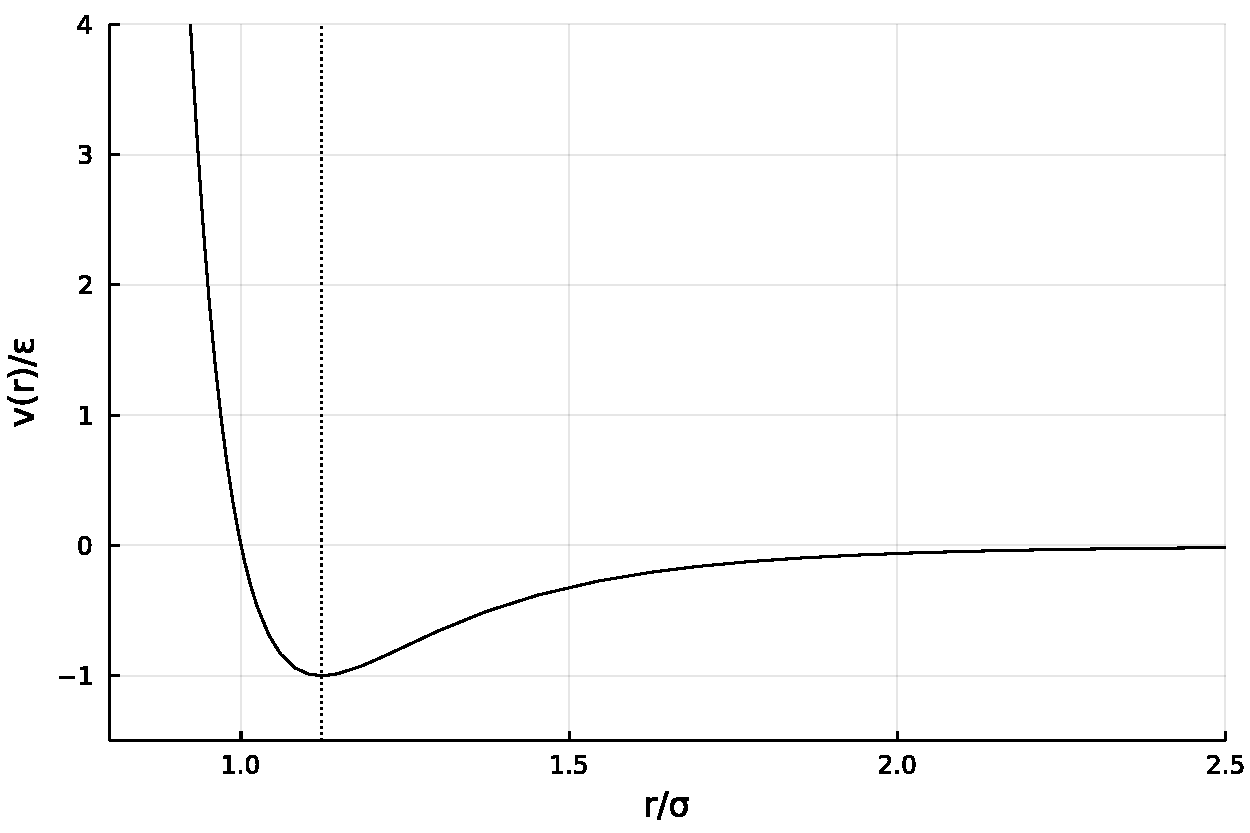
\includegraphics[width=0.7\linewidth]{figures/chapter1/lennard_jones.pdf}
      \caption{ \label{fig:lennard_jones}
        The pair potential $v$, with distances and energy given in reduced units. The equilibrium interparticular distance is indicated by the vertical dotted line.
      }
    \end{center}
  \end{figure}

\subsection{Reduced units}
It is convenient, given an atomic system, to describe quantities therein within a system of units in which they are of order one. This has several advantages. 
Firstly, like any reasonable system of units, reduced units make quantities easier and more intuitive to reason about.
Secondly, from the computational point of view, numerical artifacts due to loss of precision at very large or very small scales and overflow errors can be avoided more often.
Thirdly, they may help transfer knowledge about one system to another. 
For instance, in the Lennard-Jones system, expressing a quantity in reduced units,
and knowing the dependency of these units on the parameters $(\varepsilon,\sigma,M)$ of the system, one can infer properties about a system with parameters $(\tilde\varepsilon,\tilde\sigma,\tilde M)$ by applying the inverse transformation, thus effectively yielding equivalence of different systems under different conditions, and sparing the cost of running redundant simulations.

We describe a general procedure to construct a set of reduced units. Our choice, although not necessarily unique, is quite natural, especially when dealing with the Lennard--Jones system.
Let us fix a reference mass $m_*$, a reference energy $\varepsilon_*$ and a reference length $\sigma _*$. Then various reference quantities can be derived by natural conversions and dimensional analysis:
\begin{align*}&t_*=\sqrt{\sigma_*^2m_*\varepsilon_*^{-1}},\tag{time}\\
    &T_*=\varepsilon_*k_B^{-1},\tag{temperature}\\
    &v_*=\sigma_*t_*^{-1},\tag{velocity}\\
    &V_*=\sigma_*^3,\tag{volume}\\
    &A_*=\sigma_*^2,\tag{area}\\
    &\rho_*=V_*^{-1},\tag{density}\\
    &F_*=m_*\sigma_*t_*^{-2},\tag{force}\\
    &P_*=F_*A_*^{-1},\tag{pressure}
\end{align*}
and one can of course go on. The point is that if $X$ is a quantity, one can obtain its reduced value $X_{\mathrm{red}}$ by dividing $X$ by the reference quantity $X_*$ which is dimensionally compatible with $X$, and which can be derived as above.
For instance, given a pressure $P$, we obtain
$$P_{\mathrm{red}}= P\sigma_*^3\varepsilon_*^{-1}.$$
Note this is an adimensional quantity. Note, also that, due to the definition of the reference temperature $T_*$ relative to the reference energy $\varepsilon_*$, energies are now commensurate to temperatures.
The Boltzmann factor, which is the conversion factor between units of temperature and units of energy simplifies when expressed in reduced units, a fact we can capture with the maxim ${k_B}*=1$. This simplifies many formulae.

For a monatomic Lennard--Jones system, a natural choice for $m_*$ is the atomic mass of the considered species. We also take $\varepsilon_*=\varepsilon$ and $\sigma_*=\sigma$ (although the equilibrium length $\sigma=2^{1/6}\sigma$ is another possible choice). In the case of Argon, we use the following values:
$$m_*=6.634 \times 10 ^{-26}\, \text{kg},\ \sigma_*=3.405 \times 10^{-10}\, \text{m},\ \varepsilon_*=1.66 \times 10^{-21}\, \text{J}.$$
Unless explicitly specified, all numerical results will be in this system of reduced units.

Once a dynamic has been prescribed, and an observable of interest as been fixed, we can describe our strategy to sample from a thermodynamic ensemble.

\subsection{Ergodic averages}
We define a process $(q_t,p_t)_{t\geq 0}$ on $\mathcal E$, either deterministic or stochastic, which is invariant for the target measure $\widetilde{\mu}$, in the following sense:
for all $t\geq 0$ and all bounded measurable observable $\varphi$, we require
\begin{equation}
    \label{eq:invariant_measure}
    \int_{\mathcal E}\E^{(q,p)}\left[ \varphi(q_t,p_t)\right]\,\widetilde{\mu}(\mathrm{d}q,\mathrm{d}p)=\int_{\mathcal E}\varphi(q,p)\,\widetilde{\mu}(\mathrm{d}q,\mathrm{d}p),
\end{equation}
where the superscript in the expectation denotes that the process has value $(q,p)$ at $t=0$, and the expectation is over realizations of $(q_t,p_t)$. In other words, this is a process which, given that its initial condition is distributed according to $\widetilde{\mu}$, remains distributed according to $\widetilde{\mu}$ at any later time. It is then natural to consider average values of $\varphi$ over the trajectories:
\begin{equation}
\label{eq:ergodic_averages}
 \widehat{\varphi}_T \defeq \frac{1}{T}\int_{0}^T \varphi(q_t,p_t)\,dt,
\end{equation}
which we may hope will converge to the target ensemble average \eqref{eq:ensemble_average}. 
The convergence of ergodic averages to the ensemble average can be shown not to hold in generality, and is something which must be proven on a case by case basis, though general criteria can be derived, see for instance \cite{K87}.
If the underlying dynamic is stochastic, then the variance of the random variables \eqref{eq:ergodic_averages} becomes an issue, which one must control by ensuring that time averages are taken over long enough trajectories. 
Furthermore, since the true invariant dynamics is in general in continuous time, one must generally devise discrete-in-time approximations to the true trajectories.
However, empirical practice shows that ergodic averages obtained from computer simulations, even for a modest number of atoms, agrees very well with experimental data for certain types of systems, and even in the absence of theoretical guarantees.
\chapter{Classical ensembles}
\section{Microcanonical averages}
\subsection{Properties of Hamiltonian dynamics}


The Hamiltonian dynamics \eqref{eq:hamiltonian_dynamics} rewrites in matrix form, writing $X_t=(q_t,p_t)$:

\begin{equation}\label{eq:hamiltonian_dynamics_matrix_form} \text d X_t=J\nabla H(X_t)\dt,\end{equation}
where $J$ is the symplectic matrix

$$J = \begin{pmatrix}
    0_{dN} & \Id_{dN}\\ -\Id_{dN} & 0_{dN}.
\end{pmatrix}$$
This will be useful to investigate properties of the Hamiltonian dynamics.
Applying the chain rule to any smooth function $\varphi: \cLs \mapsto \R$, we obtain
        $$ \text d \varphi(X_t)= \text d X_t^{\intercal} \nabla \varphi(X_t)=(J \nabla H(X_t))^\intercal \nabla \varphi(X_t)\dt=(\nabla_p H \cdot \nabla_q - \nabla_q H \cdot \nabla_p)\varphi(X_t)\dt$$
        This motivates the following.
        \begin{definition}[Generator of the Hamiltonian dynamics]
            We define the generator associated with the Hamiltonian dynamics to be the operator $\cL_{\text{H}}$ defined on smooth functions by
        \begin{equation}
            \label{eq:hamiltonian_generator}
            \cL_{\mathrm{ham}}\varphi=(\nabla_p H \cdot \nabla_q - \nabla_q H \cdot \nabla_p)\varphi=\left(J\nabla H\right)^\intercal \nabla \varphi
        \end{equation}
    \end{definition}
    We can split the generator as the sum of two elementary operators,
    $$\cLham=A+B,$$
    with
    \begin{equation}
        \label{eq:Lham_splitting}
        A=\left(M^{-1}p\right)\cdot \nabla_q \qquad B=-\nabla V(q)\cdot \nabla_p.
    \end{equation}
    The generator allows us to quantify the rate of change of an observable $\varphi$ under the evolution of the system. If we define, for $t\geq 0$, the evolution operators 
    $$P_t \varphi (q_0,p_0) = \varphi(\Phi_t(q_0,p_0)),$$
where $\Phi$ is the flow associated with the Hamiltonian dynamics, that is the collection of maps $(\Phi_t)_{t\geq 0}$, defined by
    $\Phi_t (q_0,p_0) = (q_t,p_t)$, the solution to \eqref{eq:hamiltonian_dynamics} with initial conditions  $(q_0,p_0)$, then we have formally:

    $$ \frac \partial{\partial t} P_t \varphi (q,p)= \partial_t \varphi(q_t,p_t)= \cLham \varphi(q_t,p_t)=\cLham P_t \varphi(q,p)=P_t\cLham \varphi(q,p).$$
    Applying $\cLham$ to $H$ immediately gives the following result.
\begin{prop}[Energy conservation]
    \begin{equation}
    \label{eq:energy_conservation} \text d H(X_t)=0
    \end{equation}
\end{prop}
This relation expresses the fact that the Hamiltonian is invariant under the flow of \eqref{eq:hamiltonian_dynamics}. This, in turn, is the mathematical translation of the physical principle of conservation of energy.
Using the fact that the Hamiltonian flow field is divergence-free,
\begin{equation}
        \label{eq:hamiltonian_flow_divergence_free}
        \mathrm{div}\left(J\nabla H\right)=\mathrm{div}_q\left(\nabla_p H\right)-\mathrm{div}_p\left(\nabla_q H\right)=0,
\end{equation}
one can show the following property, famously known as Liouville's theorem.
\begin{prop}[Conservation of volume]
    For any measurable set $D\subset \mathcal E$, we have
    \begin{equation}
        \label{eq:conservation_of_volume}
        |\Phi_t(D)|=|D|.
    \end{equation}
\end{prop}

\begin{definition}[Symplecticity]
    A mapping $\varphi$ from $\R^{2d}$ to itself is said to be symplectic on some open set $U\subset \R^{2d}$ if it is $C^1$ and if, for all $(q,p)\in U$,
    \[\nabla \varphi^\intercal J\nabla \varphi=J,\]
    where $\nabla \varphi$ is the Jacobian matrix of $\varphi$ \eqref{eq:jacobian}.
\end{definition}

\begin{prop}
    For any $t\in \R$, the Hamiltonian flow $Phi_t$ is symplectic.
\end{prop}
Consider the momentum-reversing map

\begin{equation}
    \label{eq:momentum_reversing}
    \cR(q,p)=(q,-p)
\end{equation}
We then have the following time symmetry property.
\begin{prop}[Time symmetry]
    \begin{equation}
        \Phi_t \circ \cR \circ \Phi_t=\Id
    \end{equation}
\end{prop}

\begin{remark}
    \label{rem:non_separable_hamiltonian}
    The property \eqref{eq:energy_conservation} is only due to the form of $J$, and not to the specific expression for $H$.
    Thus any $H$, we may consider any dynamics of the form \eqref{eq:hamiltonian_dynamics_matrix_form}, to devise a dynamical system whose orbits are restricted to the level set $H^{-1}\{H(q_0,p_0)\}$.\\
    Conversely, given a differential dynamical system, if through a change of coordinates one is able to write the system under this form, one has found a conservation law.
\end{remark}

    An important remark is that if one considers each part of \eqref{eq:Lham_splitting} as a generator in itself, the corresponding dynamics is analytically solvable.
    \begin{remark}
        \label{rem:Lham_splitting_semigroups}
        Consider the two dynamics defined by
        \begin{equation}
            \label{eq:Lham_splitting_dynamics}
            \left\{\begin{aligned}
                &\dif q_t^A=M^{-1}p_t^A\dif t, &\dif p_t^A=0,\\
                &\dif q_t^B=0, &\dif p_t^B=-\nabla V(q_t^B)\dif t.
            \end{aligned}\right.
        \end{equation}
        These are easily solved, namely
        \begin{equation}
            \label{eq:Lham_splitting_dynamics_solved}
            \left\{\begin{aligned}
                &\left(q_t^A,p_t^A\right)=\left(q_0^A+tp_0^A,p_0^A\right),\\
                &\left(q_t^B,p_t^B\right)=\left(q_0^B,p_0^B-tV\left(q_0^B\right)\right).
            \end{aligned}\right.
        \end{equation}
        Moreover, these evolutions are of Hamiltonian form, with Hamiltonians corresponding respectively to the kinetic part and the configurational part only, and have corresponding generators $A$ and $B$.
        We denote by $\left(\Phi^A_t\right)_{t\geq 0}$ and $\left(\Phi^B_t\right)_{t\geq 0}$ their respective flows. This splitting property will prove useful in constructing numerical schemes for both Hamiltonian and stochastic dynamics.
    \end{remark}

    \subsection{Numerical schemes for Hamiltonian dynamics}

    It is impossible, except for a very restricted class of systems, which do not occur in practical settings anyhow, to analytically integrate Hamilton's equation \eqref{eq:hamiltonian_dynamics}. For this reason, one must revert to numerical schemes, which we may interpret as discrete approximations of the Hamiltonian flow.
    More precisely, for a fixed timestep $\Delta t$, if we possess an approximation of the flow 
    \[\tilde\Phi_{\Delta t}\approx\Phi_{\Delta t},\]
    we will deduce approximations of the evolution
    \begin{equation}\label{eq:discrete_dynamics}(q^n,p^n)\defeq \tilde\Phi_{\Delta t}^n(q_0,p_0)\approx (q_{n\Delta t},p_{n\Delta t}),\end{equation}
    which can then be used as sample points for the computation of empirical averages, discrete counterparts to the ergodic averages \eqref{eq:ergodic_averages},
    \begin{equation}
        \label{eq:discrete_ergodic_averages}
        \frac 1n\sum_{k=0}^n \varphi(q^n,p^n).
    \end{equation}
    In most common applications, the aim is to approximate the exact solution of an evolution equation as precisely as possible over a given time domain.
    In the case of molecular dynamics, however, the time domain is usually very large, because simulating long trajectories is a requirement to ensure that a representative portion of phase space is explored. As a consequence, it is in practice impossible to obtain precise solutions over a long time, because of the evolution's sensitivity to the initial conditions. 
    Furthermore, one does not even care about the exact evolution, since the dynamics are merely used as a sampling device. Instead, one key requirement is that the dynamics stay on or close to the constant Hamiltonian manifold associated with the initial conditions. It can be shown through eigenanalysis that for simple linear systems, this requirement is not satisfied by standard ODE numerical methods such as the explicit and implicit Euler schemes, or the RK4 method, for which the energy may explode or implode geometrically.
    This has the practical effect that for reasonably sized atomic systems, numerical instabilities render the simulations nonsensical after only a few time steps, a far cry from what is needed to obtain good estimates.
    One must then devise dedicated numerical methods, guided by the aim to preserve qualitative properties of the Hamiltonian evolution. It turns out that splitting schemes, based on operator splitting approximations of the Hamiltonian evolution operator over one timestep, preserve crucial qualitative properties of the Hamiltonian evolution.
    Let us fix a timestep $\Delta t>0$. Numerical schemes aim to approximate the flow $\Phi_{\Delta t}$. Splitting schemes rely on the splitting property \eqref{eq:Lham_splitting_dynamics_solved} to construct computable approximations
    \[\Phi_{\Delta t}\approx \Phi^{G_k}_{\Delta t_k}\circ \dotsm \circ \Phi^{G_1}_{\Delta t_1},\]
    where $G_i\in\{A,B\}$ for all $i$. We will be considering three schemes, the simplest of which are the symplectic Euler schemes.
    
    The symplectic Euler schemes are defined by the following update equations.
    
    \begin{equation}\label{eq:symplectic_euler_A}
    \left\{\begin{aligned}
         p^{n+1} &=p^n -\nabla V(q^n)\Delta t\\
         q^{n+1} &=q^n + M^{-1}p^{n+1}\Delta t
    \end{aligned}\right.
    \end{equation}

    \begin{equation}\label{eq:symplectic_euler_B}
        \left\{\begin{aligned}
             q^{n+1} &=q^n +M^{-1}p^n\Delta t\\
             p^{n+1} &=p^n - \nabla V(q^{n+1})\Delta t
        \end{aligned}\right.
    \end{equation}

    These correspond respectively to the splitting approximations 
    \[\Phi_{\Delta t}\approx \Phi_{\Delta t}^A\circ\Phi_{\Delta t}^B\defeq \Phi_{\Delta t}^{BA}\]
    and
    \[\Phi_{\Delta t}\approx \Phi_{\Delta t}^B\circ\Phi_{\Delta t}^A\defeq \Phi_{\Delta t}^{AB}.\]
    
    The velocity Verlet scheme is based on the splitting
    \[\Phi_{\Delta t}\approx \Phi_{\Delta t/2}^B\circ\Phi_{\Delta t}^A\circ\Phi_{\Delta t/2}^B\defeq \Phi_{\Delta t}^{BAB}.\]
    Its update equation is given by
    \begin{equation}\label{eq:verlet}
        \left\{\begin{aligned}
             p^{n+\frac12} &=p^n -\frac{\Delta t}{2}\nabla V(q^n)\\
             q^{n+1} &=q^n + \Delta t M^{-1}p^{n+\frac 12}\\
             p^{n+1} &= p^{n+\frac12}-\frac{\Delta t}{2}\nabla V(q^{n+1}).
        \end{aligned}\right.
    \end{equation}
    \subsection{Properties of symplectic schemes}
    The main interest of these schemes is that, as hinted at above, they preserve some qualitative properties of Hamiltonian dynamics, which are essential if the aim is to compute ergodic averages.
    One, which relies on the simple observation that the composition of two symplectic mappings is symplectic, is the following proposition.

    \begin{prop}
        \label{prop:symplecticity_of_schemes}
        The mappings $\Phi_{\Delta t}^{AB}$, $\Phi_{\Delta t}^{BA}$ and $\Phi_{\Delta t}^{BAB}$ are symplectic, like any mapping obtained by composition of the Hamiltonian flows $\Phi_\Dt^A$ and $\Phi_\Dt^B$.
    \end{prop}

    One may ideally wish to guarantee that the Hamiltonian is preserved under the discrete evolution induced by these schemes. This, it turns out, is too high a hope.
    It happens, however, that, for each of these schemes, an approximate Hamiltonian is (almost) exactly conserved, which we can interpret to mean that the discrete dynamics \eqref{eq:discrete_dynamics} are (almost) exact sample points for a modified dynamics, corresponding to the modified Hamiltonian.
    The order of this modification in the timestep $\Delta t$ then allows one to deduce the order of conservation of the original Hamiltonian. The proofs of this type of results fall under the umbrella of backward numerical analysis. For more information, refer to \cite{HLG03}.
    A precise statement is the following.

    \begin{figure}[htbp]
        \begin{center}
          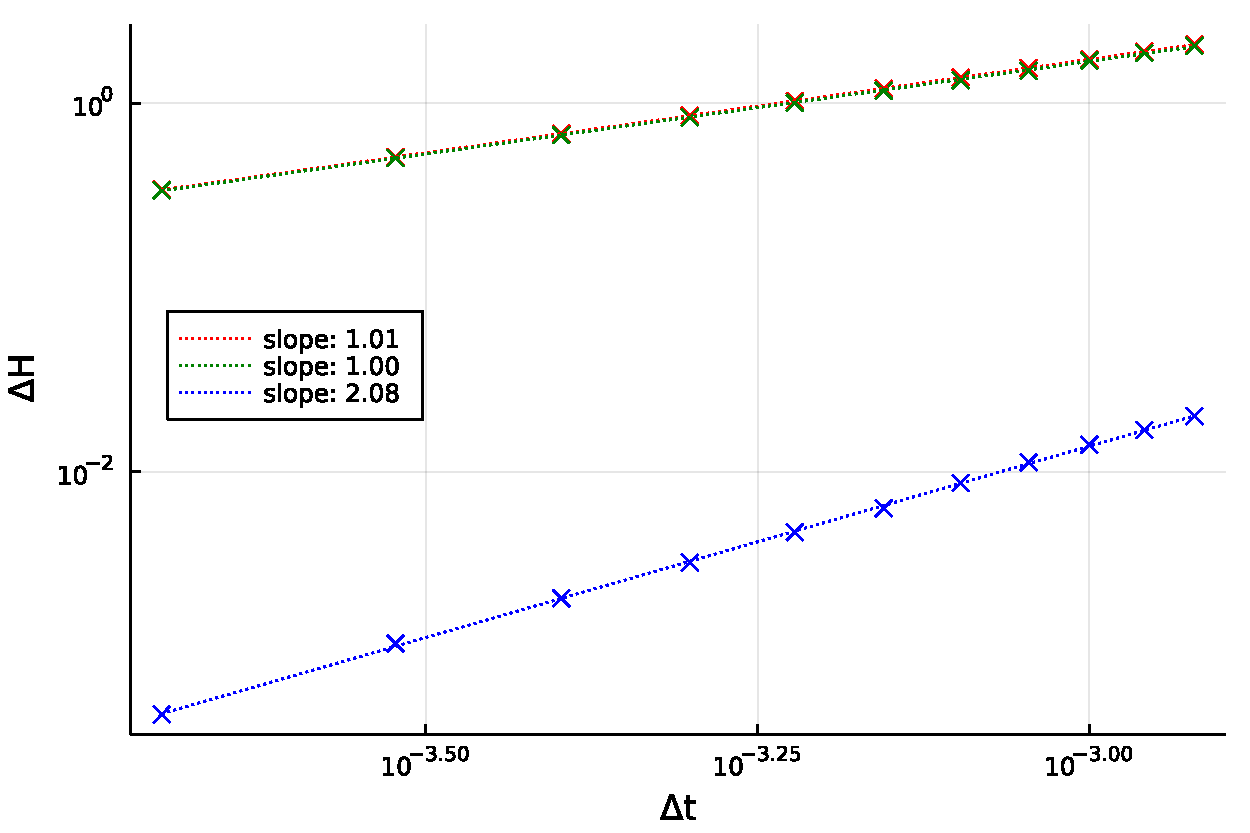
\includegraphics[width=0.7\linewidth]{figures/chapter1/hamiltonian_conservation.pdf}
          \caption{ \label{fig:hamiltonian_conservation}
            Effect of the time step on absolute variation of the Hamiltonian for the symplectic Euler (red and green) and the Verlet (blue) schemes. As expected, total variation scales as $\Delta t$ for symplectic Euler, and as $\Delta t^2$ for Verlet.
          }
        \end{center}
      \end{figure}
        
    \subsection{Shortcomings of the Hamiltonian approach}

\section{Canonical averages}

\subsection{Langevin dynamics}
We consider a special case of the inertial Langevin dynamics, defined by the following stochastic differential equation (SDE), where $\gamma, \beta$ are fixed positive constants.

\begin{equation}
    \label{eq:langevin}
    \left\{\begin{aligned}
        \text dq_t&=M^{-1}p_t\dt,\\
        \text dp_t&= -\nabla V(q_t)\dt -\gamma M^{-1}p_t\dt+\sqrt{\frac{2\gamma}\beta}\text dW_t,
    \end{aligned}\right.
\end{equation}

where $(W_t)_{t\geq 0}$ is a standard $dN$-dimensional Brownian motion.
This process is a combination of a Hamiltonian evolution with an additional action on the momenta which, if isolated, defines a $dN$-dimensional Ornstein-Uhlenbeck process.\\
This additional term be interpreted physically as the combination of two effects: a dissipation term 
$$-\gamma M^{-1}p_t\dt,$$
which can be understood as the effect of a viscous friction force on the particles, and a fluctuation term, 
$$\sqrt{\frac{2\gamma}\beta}\text dW_t,$$
which corresponds to the input of kinetic energy into the system as thermal agitation induced by a surrounding heat bath at temperature $1/(k_B\beta)$.\\
However, the physical meaning can be forgotten thanks to the fact that, \textit{in fine}, we only require that the canonical measure be invariant under this dynamic: as we shall shortly see, this is indeed the case.

\begin{remark}
    There are several ways to generalize this process: one is to consider more general, possibly non-separable, Hamiltonians, as in Remark \ref{rem:non_separable_hamiltonian}, rather than the classical Hamiltonian used above.
    The other is to allow the fluctuation-dissipation term to be parametrized by coefficients $\gamma$ and $\sigma$ depending on the state variable, and which obey a relation ensuring the invariance of $\mu$.
    Hence in full generality, we could consider the following Langevin dynamic:
    
    \begin{equation}
        \label{eq:general_langevin}
        \left\{\begin{aligned}
            \text dq_t &=\nabla_p H(q_t,p_t)\dt,\\
            \text dp_t &= -\nabla_q H(q_t,p_t)\dt -\gamma(q_t,p_t)\nabla_pH(q_t,p_t)\dt+\sigma(q_t,p_t)\rm{d}W_t.
        \end{aligned}\right.
    \end{equation}
\end{remark}
The generator of the Langevin dynamics is the operator
\begin{equation}
  \label{eq:langevin_generator}
\mathcal L_\gamma=M^{-1}p\cdot \nabla_q-\nabla V(q) \cdot \nabla_p- \gamma M^{-1} p \cdot \nabla_p+\frac\gamma\beta \Delta_p,
\end{equation}
which splits into three elementary generators, namely 
$$\mathcal L_\gamma= A+B+\gamma C=\cLham +\gamma C,$$
with
\begin{equation}
  \label{eq:C_definition}
C=-M^{-1}p\cdot \nabla_p +\frac1\beta \Delta_p.
\end{equation}
These generators individually give rise to dynamics which we can express explicitly, defined by the following evolution operators:

\begin{equation}
  \label{eq:propagators}
  \left\{\begin{aligned}
    &\mathrm{e}^{tA}\varphi(q,p)=\varphi(q+tM^{-1}p,p),\\
    &\mathrm{e}^{tB}\varphi(q,p)=\varphi(q,p-t\nabla V(q)),\\
   &\mathrm{e}^{t\gamma C}\varphi(q,p)=\mathbbm E \left[\varphi \left(q, \mathrm e^{-\gamma M^{-1}t}p + \sqrt{\frac{M}{\beta}(1-\mathrm{e}^{-2\gamma M^{-1}t})}G\right)\right],
\end{aligned}\right.
\end{equation}
where $G$ is a standard $dN$-dimensional Gaussian. The third equality translates an equality in law between an Itô integral and a Gaussian random variable, and follows by applying Itô's formula to the rescaled process
$$\e^{\gamma M^{-1}t}X_t,$$
where $X_t$ is the Ornstein-Uhlenbeck process:
\begin{equation}
    \dif X_t=-\gamma M^{-1}X_t\dif t+\sqrt{\frac{2\gamma}{\beta}}\dif W_t.
\end{equation}
 The dynamics associated with the A and B part are deterministic Hamiltonian dynamics already identified in \eqref{eq:Lham_splitting_dynamics_solved}.

\subsection{Properties of the Langevin dynamics}

    \subsubsection*{Invariance of the canonical measure}

    Using the generator, one can easily express the evolution of a probability distribution under the Langevin dynamics.
    We assume that the solution $(q_t,p_t)_{t\geq 0}$ to \eqref{eq:langevin} has a distribution with a smooth density $\rho_0$ over $\mathcal E$ at time $t=0$, and denote $\rho_t$ the probability density of $(q_t,p_t)$.
    For any test observable $\varphi$, we have
    $$\int_{\mathcal E}\varphi(q,p)\rho_t(q,p)\dif q\dif p=\int_{\mathcal E}\E^{(q,p)}\left[\varphi(q_t,p_t)\right]\rho_0(q,p)\dif q\dif p=\int_{\mathcal E}\mathrm{e}^{t\cL_\gamma}\varphi(q,p)\rho_0(q,p)\dif q\dif p,$$
    where the superscript is as in \eqref{eq:invariant_measure}. Thus,
    $$\frac{\partial}{\partial t}\int_{\mathcal E}\varphi(q,p)\rho_t(q,p)\dif q\dif p=\int_{\mathcal E}\mathrm{e}^{t\cL_\gamma}\cL\varphi(q,p)\rho_0(q,p)\dif q\dif p=\int_{\mathcal E}\cL_\gamma\varphi(q,p)\rho_t(q,p)\dif q \dif p$$
    If we define $\cL_\gamma^\dagger$ as the adjoint of $\cL_\gamma$ on the flat space $L^2(\mathcal E)$, that is,
    \begin{equation}
        \label{eq:L_dagger}
        \int_{\mathcal E}\cL_\gamma\varphi \psi=\int_{\mathcal E}\varphi \cL_\gamma^\dagger \psi \qquad\text{for all test functions }\phi,\,\psi,
    \end{equation}
    we have the Fokker-Planck equation,
    \begin{equation}\label{eq:fokker_planck}
        \frac{\partial}{\partial t}\int_{\mathcal E}\varphi(q,p)\rho_t(q,p)\dif q\dif p=\int_{\mathcal E}\varphi(q,p)\cL_\gamma^\dagger\rho_t(q,p)\dif q \dif p,
    \end{equation}
    which rewrites formally as 
    \begin{equation}
        \label{eq:fokker_planck_formal}
        \frac{\partial}{\partial t}\rho_t=\cL_\gamma^\dagger\rho_t.
    \end{equation}
    Using this equation, we can easily show that the canonical distribution is invariant under this dynamics, which is equivalent to the condition 
    $$\cL_\gamma^\dagger \mu=0.$$
    In fact, it is useful to reformulate this condition in the weighted space $L^{2}(\mu)$. Indeed, the stationary Fokker-Planck equation rewrites
    $$\int_{\mathcal E}\cL_\gamma \varphi \dif \mu=0\qquad \forall\,\varphi,$$
    or
    $$\int_{\mathcal E}\left(\cL_\gamma^* \1_{\mathcal E}\right)\varphi \dif \mu\qquad\forall\,\varphi,$$
    where $\cL_\gamma^*$ is the adjoint of $\cL_\gamma$ in $L^2(\mu)$ under the scalar product
    $$\langle \varphi,\psi \rangle_\mu\defeq \int_{\mathcal E}\varphi \psi \dif \mu.$$
    This, in turn, follows easily from the following lemma.
    \begin{lemma}
        \label{lemma:star_adjoints_langevin}
        The $L^2(\mu)$ adjoints of the elementary differential operators are given by the formulae
        \begin{equation}
            \label{eq:star_adjoints_langevin}
            \left\{\begin{aligned}
            &\partial_{q_i}^*=-\partial_{q_i}+\beta\partial_{q_i}V,\\
            &\partial_{p_i}^*=-\partial_{p_i}+\beta\left(M^{-1}p\right)_i.
            \end{aligned}\right.
        \end{equation}
    \end{lemma}
    These are easily found by integration by parts. In particular, we find that 
    $$\partial_{q_i}\partial_{p_i}^*-\partial_{p_i}\partial_{q_i}^*=\beta\left((M^{-1}p)_i\partial_{q_i}-\partial_{q_i}V\partial_{p_i}\right),$$
    whence, by summing over $i$, we get 
    \begin{equation}
        \label{eq:L_ham_antisymmetric}
        \cLham=\frac1\beta\left(\nabla_q\cdot\nabla_p^*-\nabla_p\cdot\nabla_q^*\right),
    \end{equation}
    which is an antisymmetric operator. Similarly,
    $$\partial_{p_i}\partial_{p_i}^*=\beta(M^{-1}p)_i\partial_{p_i}-\partial_{p_i}^2,$$
    hence
    \begin{equation}
        \label{eq:C_symmetric}
        C=-\frac{1}\beta\nabla_p\cdot\nabla_p^*,
    \end{equation}
    which is a symmetric operator. In summary, we have that 
    \begin{equation}
        \label{eq:L_star}
        \cL_\gamma^*=-\cLham+\gamma C=-(A+B)+\gamma C.
    \end{equation}
    It follows immediately that $\cL_\gamma^*\1_{\mathcal E}=0$. Notice that since $\cLham^*\1_{\mathcal E}=0$, the canonical measure is also invariant under the Hamiltonian dynamics. However, because of the energy conservation property \eqref{eq:energy_conservation}, ergodic averages cannot in general converge to their averages under $\mu$.

    \subsubsection{Convergence to equilibrium}

\subsection{Overdamped limit of Langevin dynamics}
    As already pointed out, the fact that the kinetic marginal of $\mu$ is a Gaussian distribution makes sampling canonical momenta trivial. 
    Instead, the main problem is sampling from $\nu$. It follows directly from the invariance of $\mu$ under trajectories of the Langevin dynamics that $\nu$ is invariant under the configurational trajectories of the Langevin dynamics.
    It would be convenient, however, to have at our disposal a dynamics on $\mathcal D$ which has $\nu$ as an invariant measure.
    It turns out this is possible, by observing that the invariance of $\mu$ is independent of the parameter $\gamma$, and taking the limit $\gamma\to\infty$. This requires some care.
    Notice the SDE on the momenta in \eqref{eq:langevin} rewrites 
    \[\dif p_t=-\nabla V(q_t)\dif t-\gamma \dif q_t+\sqrt{\frac{2\gamma}\beta}\dif W_t,\]
    thus integrating gives
    \[q_t-q_0=\frac{p_0-p_t}\gamma -\frac{1}\gamma\int_0^t\nabla V(q_s)\dif s +\sqrt{\frac{2}{\gamma\beta}}W_t.\]
    The scaling invariance of the Brownian motion $(\sqrt{\alpha}W_{t/\alpha^2})_{t\geq 0}\sim (W_t)_{t\geq 0}$ suggests considering the timescale $\gamma\beta t$, thus
    \[q_{\gamma\beta t}-q_0=\frac{p_0-p_{\gamma\beta t}}\gamma-\frac1{\gamma}\int_0^{\gamma\beta t}\nabla V(q_s)\dif s +\sqrt{2}\tilde{W_t},\]
    where $\tilde W$ is again a Brownian motion. Using the change of variables $s=\gamma \beta u$ in the integral term yields
    \begin{equation}\label{eq:rescaled_langevin}q_{\gamma\beta t}-q_0=\frac{p_0-p_{\gamma\beta t}}\gamma-\beta\int_0^{t}\nabla V(q_{\gamma\beta u})\dif u +\sqrt{2}\tilde{W_t},\end{equation}
    At this point, we formally take $\gamma\to\infty$, which suggests the following SDE for the rescaled in time process,
    \begin{equation}
        \label{eq:overdamped_langevin}
        \dif q_t=-\beta \nabla V(q_t)\dif t+\sqrt{2}\dif W_t.
    \end{equation}
    
    This equation defines the overdamped Langevin, or Brownian, dynamics.
    To justify the limit in a rigorous manner, one would hope to show that the rescaled process \eqref{eq:rescaled_langevin} converges in law to a weak solution of the SDE \eqref{eq:overdamped_langevin}, in some functional space.
    However, this is technical overkill, since, we only need to consider dynamics as sampling devices. In fact, the physical interpretation of this equation is not even clear in terms of the dimensions of the quantities at play.
    We can just as well take equation \eqref{eq:overdamped_langevin} as given, and be satisfied by the following fact.

    \begin{prop}
        The configurational Gibbs measure $\nu$ is invariant under the dynamics \eqref{eq:overdamped_langevin}.
    \end{prop}

    This result follows along the same lines as for the Langevin dynamics. The generator (now acting on functions with domain $\mathcal D$) is the operator
    \begin{equation}
        \label{eq:overdamped_langevin_generator}
        \cL\varphi=-\beta\nabla V\cdot \nabla\varphi + \Delta \varphi.
    \end{equation}
    Again, we consider the weighted space $L^2(\nu)$. Adjoints of elementary differential operators are still given by the first line of \eqref{eq:star_adjoints_langevin}, and it is then easily seen that
    \begin{equation}
        \label{eq:L_overdamped_symmetric}
        \cL=-\nabla^*\cdot\nabla
    \end{equation}
    is a symmetric operator. Again we have $\cL^*\1_{\mathcal D}=0$, so $\nu$ satisfies the stationary Fokker-Planck equation under this dynamics.

    \begin{remark}
        Instead of rescaling time by $\beta\gamma$, we could have rescaled by $\gamma$, which would yield the dynamics
        \begin{equation}
            \label{eq:overdamped_langevin_alt}
            \dif q_t=-\nabla V(q_t)\dif t+\sqrt{\frac 2\gamma}\dif W_t.
        \end{equation}
        Which formulation to choose is a matter of preference, since both yield a dynamics invariant under $\nu$, as seen from the identity (where we still write $\cL$ for the generator)
        \[\cL=-\frac1\beta\nabla^*\cdot\nabla.\]
    \end{remark}

    As for the Langevin dynamics, it is possible to show tha


\subsection{Splitting schemes for the Langevin dynamics}
Just as in the Hamiltonian case, we can define schemes for the Langevin dynamics based on approximating the evolution operator over one timestep by splitting the generator $\cL_\gamma$, and combining the corresponding evolution operators \eqref{eq:propagators} in a sequence.
We refer to such a splitting approximation by the sequence in which the individual propagators are composed. It is useful at this point to introduce the stochastic flow map associated with the Ornstein-Uhlenbeck dynamics.
\begin{equation}
    \label{eq:stochastic_flow_c}
    \Phi_t^C(q,p,\xi)=\left(q, \mathrm e^{-\gamma M^{-1}t}p + \sqrt{\frac{M}{\beta}(1-\mathrm{e}^{-2\gamma M^{-1}t})}\xi\right),
\end{equation}
where $\xi\in \R^{dN}$, the point being $\E[\varphi\left(\Phi_t^C(q,p,G)\right)]=\mathrm{e}^{t\gamma C}\varphi(q,p)$ when $G$ is standard Gaussian.
Given an ordering of operators, 
\begin{equation}\label{eq:splitting_ordering}(R_1,\dots,R_k)\in \{A,B,\gamma C\}^k,\end{equation}
we can consider the mapping, which we note, by a slight abuse, as
\begin{equation}\label{eq:markov_mapping}\Phi^{R_1,\dots R_k}\defeq\Phi_{\Delta t/n_{R_k}}^{R_k}\circ\dots\circ\Phi_{\Delta t/n_{R_1}}^{R_1},
\end{equation}
where
$$n_R\defeq \#\left\{1\leq j\leq n \middle| R_j=R\right\}$$
for $R\in\{A,B,\gamma C\}$, and which we define to be the mapping which takes a point in phase space and $n_{\gamma C}$ vectors in $\R^{dN}$ $(\xi_1,\dots,\xi_{n_{\gamma C}})$, yielding a point in phase space by successively applying the flow, and, if need be, stochastic flow, mappings corresponding to the reverse ordering of \eqref{eq:splitting_ordering}.
Applying this mapping with a vector of independent standard Gaussians yields a stochastic mapping, which defines the update rule for the splitting scheme associated with the ordering \eqref{eq:splitting_ordering}.
An important property which follows from writing the update rule using the mapping \eqref{eq:markov_mapping} is that numerical trajectories formed by iterating this update rule with independent vectors of standard Gaussians form a Markov chain.
The hope is that the invariant measure corresponding to this Markov chain (provided it is unique) is a close approximation to the canonical measure, as well as being ergodic.

We will refer to such schemes by the name obtained by concatenating the names of each operator appearing in the ordering, using $O$ instead of $\gamma C$.
For instance, the BAO scheme is given by the following update rule, which corresponds to applying the symplectic Euler scheme over one timestep, followed by one timestep of the Ornstein-Uhlenbeck stochastic flow \eqref{eq:stochastic_flow_c}.

    \begin{example}[BAO scheme]
        The update rule is given by the following equations, where we introduce the intermediate momentum variable $p^{n+\frac12}$:
        \begin{equation}\label{bao}
            \left\{\begin{aligned}
                 p^{n+\frac12} &=p^n -\Delta t\nabla V(q^n)\\
                 q^{n+1} &=q^n + \Delta t M^{-1}p^{n+\frac 12}\\
                 p^{n+1} &= \alpha_{\Delta t}p^{n+\frac12}+\sigma_{\Delta t}G^n,
            \end{aligned}\right.
        \end{equation}
        where $G^n$ is a standard $dN$-dimensional Gaussian.
    \end{example}
    Similarly, we define the BAOAB scheme.
    \begin{example}[BAOAB scheme]
        The update rule is given by the following equations, with additional intermediate coordinate and momentum variables:
        \begin{equation}\label{baoab}
            \left\{\begin{aligned}
                 p^{n+\frac13} &=p^n -\frac{\Delta t}{2}\nabla V(q^n)\\
                 q^{n+\frac12} &=q^n + \frac{\Delta t}{2} M^{-1}p^{n+\frac 13}\\
                 p^{n+\frac23} &=\alpha_{\Delta t}p^{n+\frac13}+\sigma_{\Delta t}G^n\\
                 q^{n+1} &=q^{n+\frac12} + \frac{\Delta t}{2} M^{-1}p^{n+\frac 23}\\
                 p^{n+1} &= p^{n+\frac23}-\frac{\Delta t}{2}\nabla V(q^{n+1}),
            \end{aligned}\right.
        \end{equation}
        where, again, $G^n$ is a standard $dN$-dimensional Gaussian.
    \end{example}
     Now we have a recipe to make an infinite number of numerical schemes, which can easily be implemented in a computer.
     We could even go further and consider methods with an uneven distribution for the secondary timesteps, the introduction of negative secondary timesteps for the $A$ and $B$ steps, and so on.
     This room for creativity highlights the need for criteria to assess the quality of such schemes. Several considerations have to be weighed.

     \begin{enumerate}[(i)]
         \item Our aim is to compute long trajectories, which are needed to ensure that phase space is properly explored, as well as to obtain better statistical properties for averages \eqref{eq:discrete_ergodic_averages}. Thus, for a fixed computational budget, we desire a scheme which allows us to take as large a timestep $\Delta t$ as possible. This is the issue of numerical stability.
         \item The use of a positive timestep $\Delta t$ implies in general that the invariant measure for the Markov chain corresponding to a given scheme is not the canonical measure. This issue is called systematic error, or bias, and one would desire a scheme which minimizes this bias.
         \item The main computational cost in computing iterates of these numerical schemes is the evaluation of the gradient of the potential used for the $B$ steps. As such, it is desirable to have a scheme which requires as few evaluations of this gradient per iteration. Some care must be taken when implementing these, to ensure that already computed gradients are not re-computed: for instance, the gradient in the last step of the BOAB scheme, is equal to the one in the first step of the next iteration.
         \item Notice that the parameter $\gamma$ is free for the practicioner to choose. A natural question is to determine the properties of the marginal dynamics in $q$ in the limit $\gamma \to +\infty$, and in particular if we obtain a consistent discretization of the overdamped Langevin dynamics.
         \item Conversely, one could ask about properties of the dynamics as we take the Hamiltonian limit $\gamma\to 0$.
     \end{enumerate}

    \subsection{Error analysis for splitting schemes}
     Let us address the second of these concerns 

    \subsection{Unbiased sampling}
     It turns out that one can devise schemes which have no systematic error: the Markov chain generating the trajectories has invariant measure exactly $\mu$.
     These methods are based on the Metropolis-Hastings algorithm, which gives a general method to sample a given target distribution.
    \subsubsection*{The Metropolis-Hastings algorithm}
     We aim to sample from a given target measure on $\R^d$. We suppose we have at our disposal a way to generate proposal points from a given point $\in\R^d$. This amounts to defining a transition kernel, the \textit{proposal}, which we may take to be a map
     \[T:\R^d\times\R^d\longrightarrow\R_+,\]
     such that for any $x\in\R^d$, $T(x,\cdot)$ is a probability density on $\R^d$, and which is cheap to sample from (very often these are taken to be some form of Gaussian distribution). We also assume that we always have $T(x,y)>0$. (This is always the case if the kernel is Gaussian).
     We also fix a function $r:\R_+\to(0,1]$, the \textit{rule}, which satisfies the property
     \begin{equation}\label{eq:mh_rule}x\cdot r\left(\frac1x\right)=r(x)\end{equation}
     We then define a Markov chain by iterating the following algorithm, starting from an arbitrary point $q^0\in \R^d$.

     \begin{algorithm}[Metropolis-Hastings]
        From a given point $q^n$
        \begin{enumerate}[(1)]
            \item Sample a proposal $\tilde q^{n+1}$ according to the probability law $T(q^n,\cdot)$.
            \item Compute\[R(\tilde q^{n+1},q^n)=r\left(\frac{\pi(\tilde q^{n+1})T(\tilde q^{n+1},q^n)}{\pi(q^n)T(q^n,\tilde q^{n+1})}\right).\]
            \item With probability $R(\tilde q^{n+1},q^n)$, set $q^{n+1}=\tilde q^{n+1}$, otherwise, set $q^{n+1}=q^n$.
            \item Go back to step (1) with $q^n\leftarrow q^{n+1}$.
        \end{enumerate}
     \end{algorithm}

    Since $T$ defines a Markov chain, we may always write $\tilde q^{n+1}=\Phi(q^n,\xi^n)$ for some family of \iid variables $(\xi^n)_{n\geq 0}$. We can then write $q^{n+1}$ in a concise form:
    \begin{equation}
        \label{eq:metropolis_hastings_algorithm}
        q^{n+1}=\Phi(q^n,\xi^n)+\1_{U^n>R\left(\Phi(q^n,\xi^n),q^n\right)}\left(q^n-\Phi(q^n,\xi^n)\right)=\Psi(q^n,\xi^n,U^n),
    \end{equation}
    where the $U^n$ are \iid uniform on $[0,1]$, such that the $(\xi^n,U^n)$ are an independent family. This shows that the algorithm defines a Markov chain. Furthermore, we may compute
    \begin{equation}
        \begin{aligned}
            \pi(x)\mathbb P\left(q^1=y \middle| q^0=x\right)&=\pi(x)T(x,y)R(x,y)\\
            &=\pi(x)T(x,y)r\left(\frac{\pi(y)T(y,x)}{\pi(x)T(x,y)}\right)\\
            &=\pi(y)T(y,x)\frac{\pi(x)T(x,y)}{\pi(y)T(y,x)}r\left(\frac{\pi(y)T(y,x)}{\pi(x)T(x,y)}\right)\\
            &=\pi(y)T(y,x)r\left(\frac{\pi(x)T(x,y)}{\pi(y)T(y,x)}\right)\ \text{(Using \eqref{eq:mh_rule})}\\
            &=\pi(y)\mathbb P\left(q^1=x\middle|q^0=y\right).
        \end{aligned}
    \end{equation}
    Thus, the chain is reversible with respect to $\pi$ which is then is an invariant measure.
    Note that the algorithm is applicable even when we do not know how to evaluate $\pi$, but only the ratios $\pi(x)/\pi(y)$, which is in particular the case for Gibbs measures.

    \begin{remark}[Rules for Metropolis-Hastings]
        Possible choices for $r$ are:
        \begin{enumerate}
            \item The Metropolis rule, \[r(x)=\min\left\{1,x\right\},\]
            \item The Barker rule, \[r(x)=\frac{x}{1+x},\]
            \item Any combination of these of the form, for $\gamma>0$, \[r(x)=\frac{x}{1+x}\left(1+2\left(\frac12\min\left(r,\frac 1r\right)\right)^\gamma\right).\]
        \end{enumerate}
    \end{remark}

    \subsubsection*{Metropolized schemes for the underdamped Langevin dynamics}
    The Metropolis-Hastings algorithm provides a general recipe to define an unbiased Markov chain for the Langevin dynamics: one only needs to specify a proposition kernel and an acceptance rule.
    In fact, 

    \begin{example}[A GHMC scheme]
        Suppose we have at our disposal i.i.d families $(U_n)_{n\geq1}$ and $(G_n)_{n\geq 1}$ where $U_1$ is uniform on $[0,1]$ and $G_1$ is a standard Gaussian in $\R^{dN}$.
            \begin{equation}\label{ghmc}
                \left\{\begin{aligned}
                     &p^{n+\frac12} =\alpha_{\Delta t}p^n +\sigma_{\Delta t}G_n\\
                     &\tilde p^{n+\frac12} =p^{n+\frac 12} - \frac{\Delta t}{2} \nabla V(q^n)\\
                     &\tilde q^{n+1} =q^n+\Delta t M^{-1} \tilde p^{n+\frac 12}\\
                     &\tilde p^{n+1} =\tilde p^{n+\frac12} - \frac{\Delta t}{2} \nabla V(\tilde q^{n+1})\\
                     &r_n \defeq \min\left\{1,\exp(-\beta(H(\tilde q^{n+1},\tilde p^{n+1})-H(q^n,p^{n+\frac12})))\right\}\\
                     &(q^{n+1},p^{n+1}) = \1_{U_n > r_n}(q^n,-p^{n+\frac12})+\1_{U_n\leq r_n}(\tilde q^{n+1},\tilde p^{n+1})
                \end{aligned}\right.
            \end{equation}
        \end{example}

\subsection{Asymptotic variance}

\begin{figure}[htbp]
    \begin{center}
      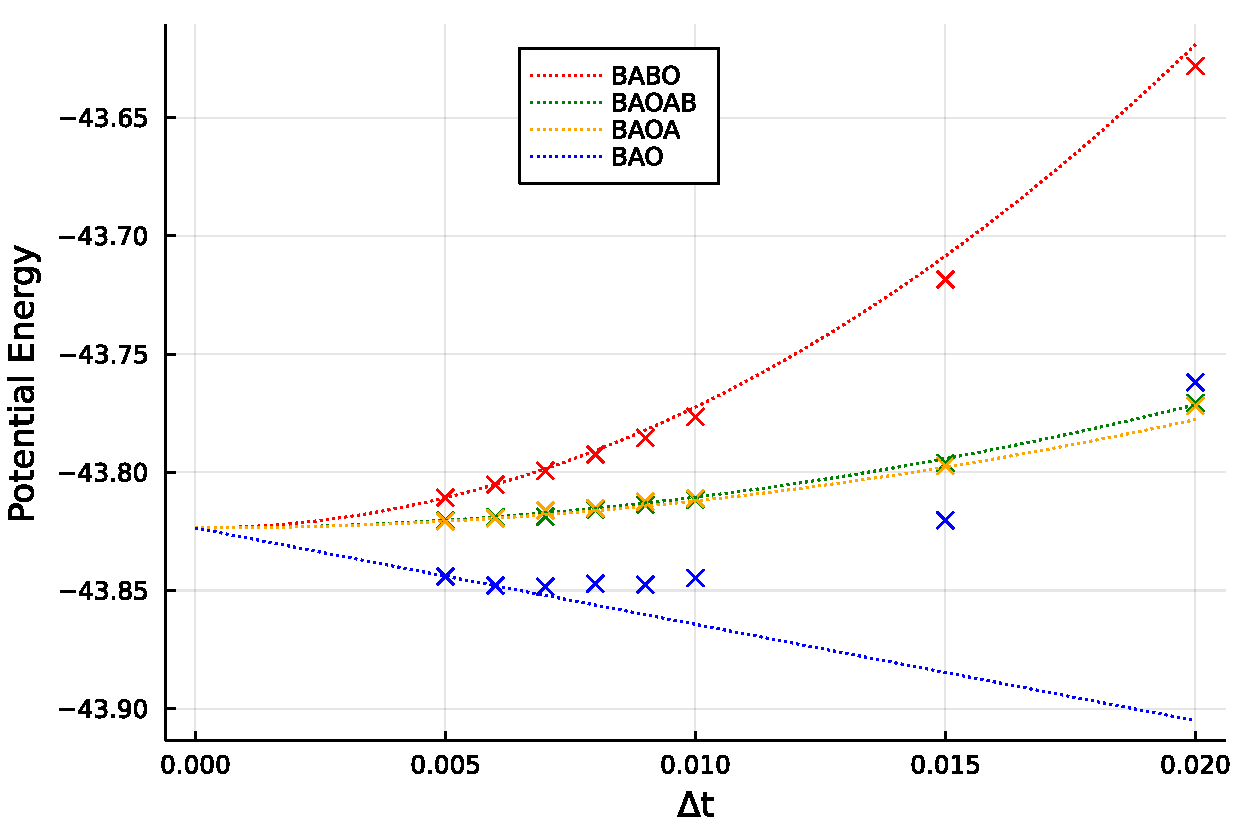
\includegraphics[width=0.49\linewidth]{figures/chapter1/potential_energy_bias.pdf}
      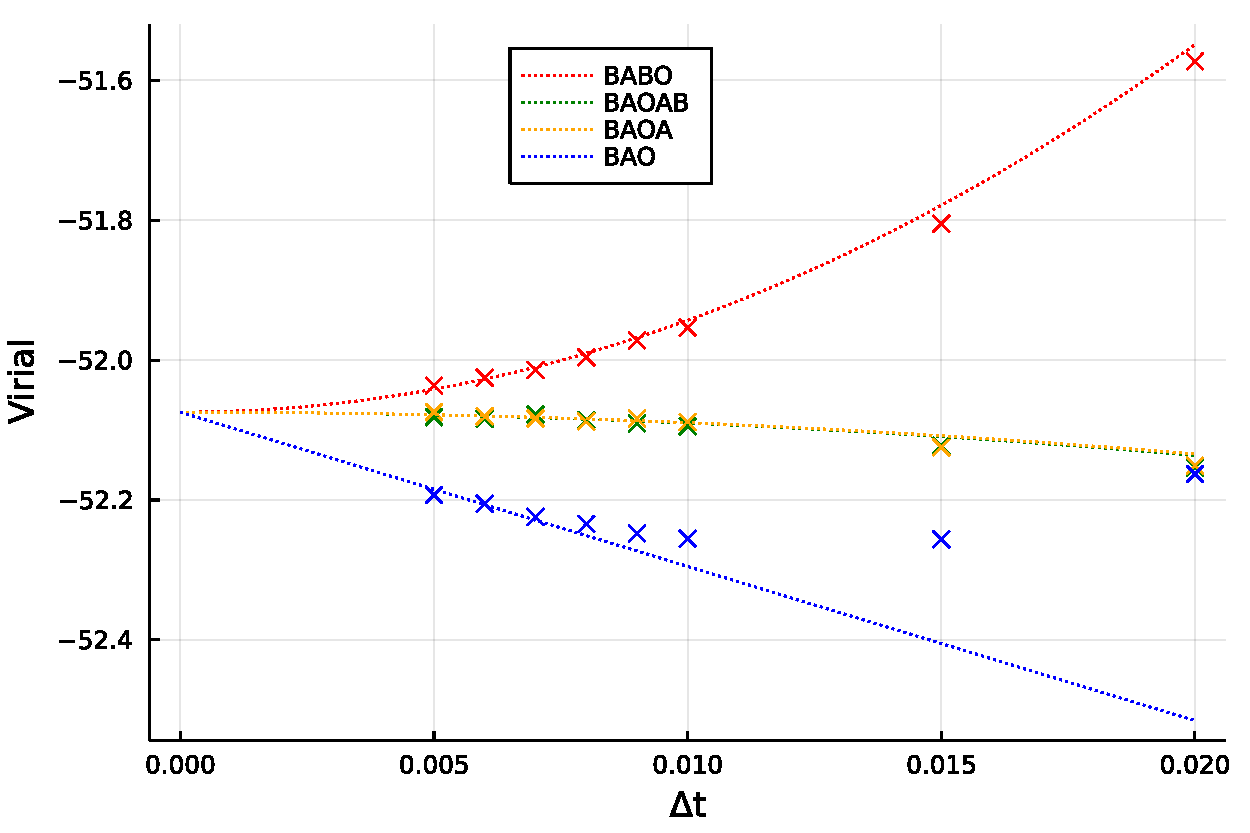
\includegraphics[width=0.49\linewidth]{figures/chapter1/virial_bias.pdf}
      \caption{ \label{fig:configurational_bias}
        Effect of the time step on average potential energy and virial for a Lennard-Jones system of 27 particles.
      }
    \end{center}
  \end{figure}

  \begin{figure}[htbp]
    \begin{center}
      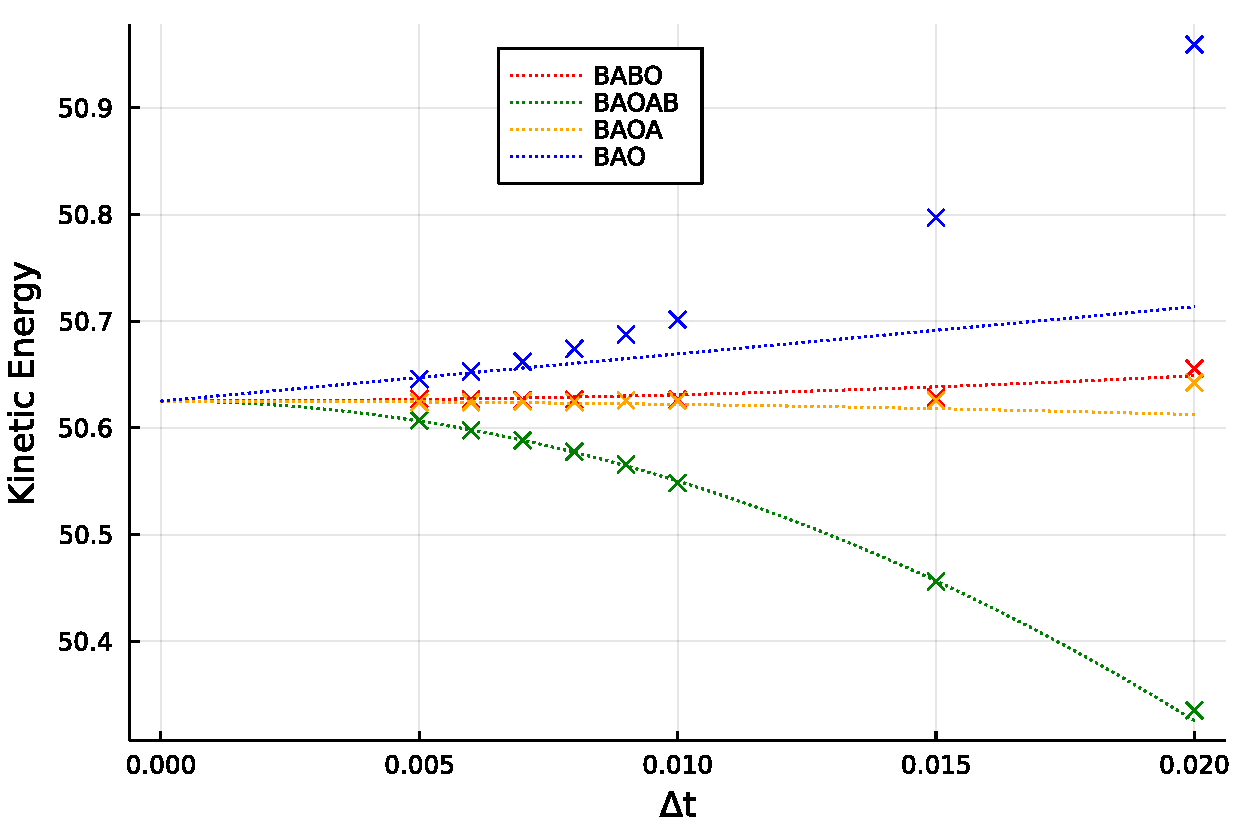
\includegraphics[width=0.7\linewidth]{figures/chapter1/kinetic_energy_bias.pdf}
      \caption{ \label{fig:kinetic_energy_bias}
        Effect of the time step on average kinetic energy for a Lennard-Jones system of 27 particles.
      }
    \end{center}
  \end{figure}

To explain the overlap of bias between the BAOAB and the BAOA schemes observed for the potential energy and virial on Figure \ref{fig:configurational bias}, we use the following result, which is a variation on the TU lemma.
\begin{lemma}\label{TU_like_lemma}
    Let $P_{\Delta t}, Q_{\Delta t}$ be bounded operators on $B^\infty(\mathcal E)$.
    Assume that, for any $n\geq 1$,
    $$ R P_{\Delta t}^n = Q_{\Delta t}^n S,$$
    where $R$ and $S$ are bounded operators on $B^\infty (\mathcal E)$, such that $R\1=\1$, and that the following ergodic condition holds: for any $\varphi \in B^\infty(\mathcal E)$, and almost all $(q,p) \in \mathcal E$,

    $$ \underset{n\to\infty}\lim P_{\Delta t}^n\varphi (q,p) = \int_{\mathcal E} \varphi(q,p)\mu_{\Delta t,P}(\text d q,\text d p) $$
    $$ \underset{n\to\infty}\lim Q_{\Delta t}^n\varphi (q,p) = \int_{\mathcal E} \varphi(q,p)\mu_{\Delta t,Q}(\text d q,\text d p).$$

    Then  we can relate $\mu_{\Delta t,P}$ and $\mu_{\Delta t,Q}$ via the following relation:

    \begin{equation}
        \label{TU_like_lemma_ccl}
    \int_{\mathcal E} \varphi(q,p) \mu_{\Delta t,P}(\text d q,\text d p)=\int_{\mathcal E} S\varphi(q,p) \mu_{\Delta t,Q}(\text d q,\text d p)
    \end{equation}
    \begin{proof}
        Fix an initial probability measure $\rho$ on $\mathcal E$, absolutely continuous with respect to the Lebesgue measure. Then we may write, using dominated convergence to pass to the limit:

        \begin{align*}
            &\int_{\mathcal E}RP_{\Delta t}^n \varphi(q,p)\rho(\text d q,\text d p)\\
            &=\int_{\mathcal E}P_{\Delta t}^n \varphi(q,p)R^{\dagger}\rho(\text d q,\text d p)\\
            &\underset{n\to\infty}{\longrightarrow}\int_{\mathcal E} \left(\int_{\mathcal E}\varphi(q,p)\mu_{\Delta t,P}(\text d q,\text d p)\right) R^\dagger \rho(\text d \tilde q,\text d \tilde p)\\
            &=\int_{\mathcal E}\varphi(q,p)\mu_{\Delta t,P}(\text d q,\text d p)\int_{\mathcal E}R\1 \text d \rho\\
            &=\int_{\mathcal E}\varphi(q,p)\mu_{\Delta t,P}(\text d q,\text d p)
        \end{align*}
        Furthermore, applying the ergodic condition to the bounded function $S\varphi$ gives

        $$ \int_{\mathcal E} Q_{\Delta t}^n (S\varphi)(q,p) \rho(\text d q,\text d p) \text d q \text d p \underset{n\to\infty}{\longrightarrow}\int_{\mathcal E} \left (\int_{\mathcal E}S\varphi(q,p)\mu_{\Delta t,Q}(\text d q,\text d p)\right)\rho(\text d \tilde q,\text d \tilde p)=\int_{\mathcal E}S\varphi(q,p)\mu_{\Delta t,Q}(\text d q,\text d p).$$

        Since $RP_{\Delta t}^n=Q_{\Delta t}^n S$, identifying the two limits yields \eqref{TU_like_lemma_ccl}
    \end{proof}
\end{lemma}

\begin{corollary}
Let $ \pi^{\mathrm{BAOA}}_{\Delta t}$ and $\pi^{\mathrm{BAOAB}}_{\Delta t}$ be the invariant measures for the Markov transition operators defined respectively by the BAOA and BAOAB schemes for a fixed timestep $\Delta t$. If the ergodic condition holds, then the corresponding marginal distributions on $\mathcal D$ are equal.

\begin{proof}
    We denote by $P_{\Delta t}$ the transition operator for the BAOA scheme, and similarly $Q_{\Delta t}$ for the BAOAB scheme. It is straightforward to check that 
    $$ \rme^{\frac{\Delta t}2 B}P_{\Delta t}^n=Q_{\Delta t}^n \rme^{\frac{\Delta t}2 B}.$$

    Assuming the ergodic condition of Lemma \ref{TU_like_lemma} (TODO reference article for sufficient conditions), we can apply the result to get, for any bounded measurable observable $\varphi$,

    $$ \int_{\mathcal E} \varphi(q,p)\pi^{\mathrm{BAOA}}_{\Delta t}(\text d q,\text d p)=\int_{\mathcal E} \rme^{\frac{\Delta t}2 B}\varphi(q,p)\pi^{\mathrm{BAOAB}}_{\Delta t}(\text d q,\text d p).$$

    Now if $\varphi (q,p)= \varphi (q,0) \defeq \varphi(q)$ for all $p$, then $\rme^{\frac{\Delta t}2 B}\varphi=\varphi$, which yields the desired conclusion:

    $$\forall \varphi \in B^\infty(\mathcal D),\ \int_{\mathcal E} \varphi(q)\pi^{\mathrm{BAOA}}_{\Delta t}(\text d q,\text d p)=\int_{\mathcal E}\varphi(q)\pi^{\mathrm{BAOAB}}_{\Delta t}(\text d q,\text d p).$$
\end{proof}

\end{corollary}

The corollary also gives a non-trivial relation between the marginal distributions in momentum space, which explains the difference displayed on (Figure \ref{fig:kinetic_energy_bias}) between those two schemes.



\subsection{Illustration: the equation of state of Argon}
\begin{figure}[htbp]
    \begin{center}
      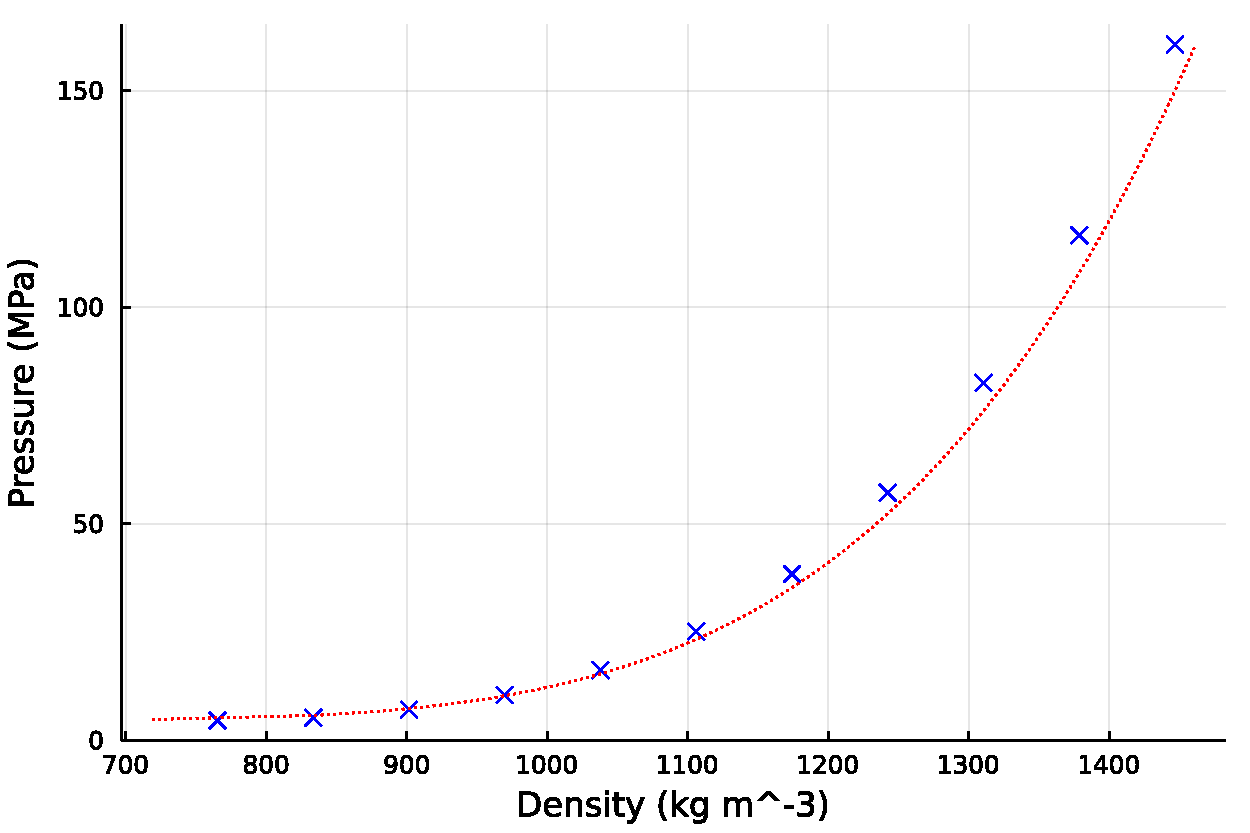
\includegraphics[width=0.49\linewidth]{figures/chapter1/argon_nvt_150K.pdf}
      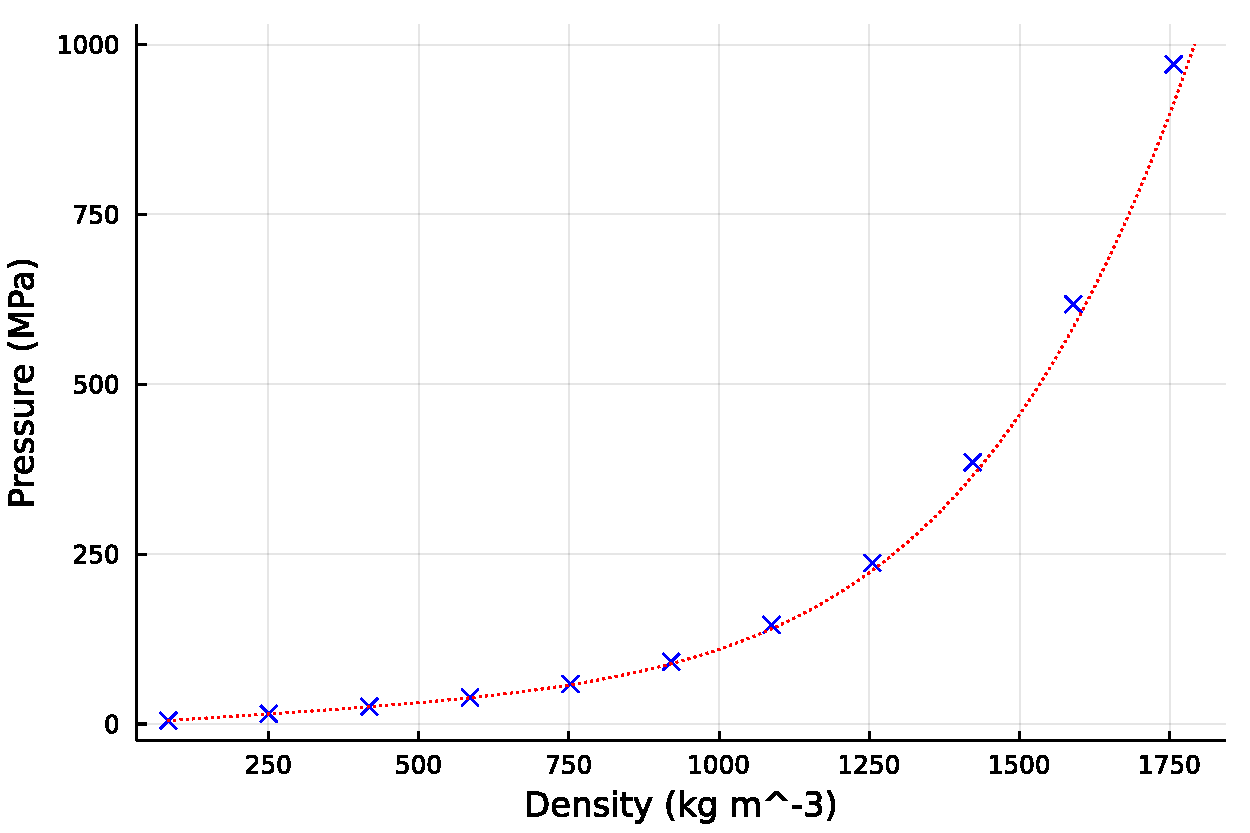
\includegraphics[width=0.49\linewidth]{figures/chapter1/argon_nvt_300K.pdf}
      \caption{ \label{fig:eos_argon}
        Simulated equations of state of Argon at 150 K (liquid phase, left) and 300 K (supercritical phase, right). Experimental reference curves are plotted in red, simulated data points are scattered in blue.
      }
    \end{center}
  \end{figure}
\chapter{Transport properties}
So far, we have only considered methods to sample static averages, which concern quantities at thermodynamic equilibrium.
Such techniques yield information about the bulk macroscopic properties of the system, for which there is no discernable macroscopic evolution.
We now turn to the next natural question, which is to consider systems in which there is such an evolution,
 which typically arises from a perturbation of the equilibrium dynamics, either by the introduction of a non-gradient forcing term, 
 or a modification of the fluctuation-dissipation part for which the fluctuation-dissipation relation \eqref{eq:general_fd_relation} is not verified.
 We will not consider the latter case, which is relevant for instance to the modelling of heat transport within an atomic system, to concentrate on the first case.
 In general, systems undergoing such a perturbation of the dynamics will reach a new steady state in which there is a net flux in some observable.
 Mathematically, this translate into the existence of a response observable $R$ which has zero average with respect to the canonical measure $\mu$, but which has a positive average with respect to the perturbation steady-state.
 A natural question is that of the sensitivity of the system to the perturbation: one way to quantify this is to modulate the strength of the perturbation by a positive real parameter $\eta>0$, and,
  assuming that the average response is asymptotically linear as $\eta\to 0$, to compute the linear coefficient linking $\eta$ and the average response. 
  This quantity is called a \textit{transport coefficient}, and we will dedicate the next two chapters to different methods of computing them using molecular simulation.

\section{Non-equilibrium molecular dynamics}
\subsection{General framework}
We first consider the most natural method, which is to directly apply a forcing term which is not the gradient of a periodic function. 
The general framework is that of a classical Langevin dynamics

\begin{equation}
    \label{eq:general_nemd_dynamics}
    \left\{\begin{aligned}
        \text dq_t&=M^{-1}p_t\dt,\\
        \text dp_t&= -\nabla V(q_t)\dt -\gamma M^{-1}p_t\dt+\sqrt{\frac{2\gamma}\beta}\text dW_t +\eta F(q_t)\dif t,
    \end{aligned}\right.
\end{equation}
perturbed by the configuration-dependent forcing term $F$, and where the strength of the perturbation is modulated by the parameter $\eta>0$.
Its generator is given by the operator 
\begin{equation}
    \label{eq:nemd_generator}
    \cL_{\gamma,F}=\cL_\gamma +\eta F\cdot \nabla_p = \cL_\gamma +\eta \widetilde{\cL}.
\end{equation}
It is also possible to consider non-equilibrium generalized Langevin equations, which are analogous perturbations of \eqref{eq:general_langevin}.
Given a response of interest $R$, the transport coefficient is given by the following definition:

\begin{equation}
    \label{eq:transport_coefficient}
    \rho_{R,F}=\underset{\eta \to 0}{\lim}\, \frac{\mathbb{E}[R]}{\eta},
\end{equation}
where $\mathbb{E}_\eta$ denotes the expectation with respect to the steady-state probability distribution. 
If the context makes $R$ clear from the knowledge of $F$, we will drop it from the notation and simply write $\rho_F$ for the transport coefficient.
For this definition to make sense, one has to show that the steady-state with respect to which we take the expectation is well-defined.
Since the steady-state is defined by the fact that it is invariant with respect to the dynamics \eqref{eq:general_nemd_dynamics}, 
this translate into the fact that it is the solution to a stationary Fokker-Planck equation, in the sense of distributions:
\begin{equation}
    \label{eq:nemd_fp_equation}
    (\cL_\gamma +\eta \widetilde{\cL})^\dagger \psi_\eta = 0,
\end{equation}
where $\psi_\eta$ is the steady state measure. Using analytic properties of $\cL_{\gamma,F}$ (such as hypoellipticity), one can hope to infer regularity results of its solutions, such as the existence of a smooth density.
Existence and unicity can in principle be inferred following Klieman's method \cite{K87}. 
The steady-state measure $\E_\eta$ is a high-dimensional measure on phase space for which a closed form is generally unavailable.
 Thus, as usual, one has to resort to ergodic averages under the dynamics \eqref{eq:general_nemd_dynamics} to compute ensemble averages.
 This poses another theoretical difficulty, that of showing that the steady-state measure is ergodic.

In fact, for our purposes, $F$ will always be $L\mathbb{T}^{dN}$-periodic, and so we can invoke a special case of Proposition 1 in \cite{JPS15} with time-constant forcings, provided $V$ and $F$ are smooth.
\begin{theorem}[Existence of a unique ergodic measure with smooth density]\label{thm:nemd_exst_invariant_measure}
    Let $\eta_*>0$. For all $\eta\in[-\eta_*,\eta_*]$, the Fokker-Planck equation \eqref{eq:nemd_fp_equation} admits a unique solution with a $C^\infty$ density $\psi_\eta$.
    Additionally, the evolution semi-group decays exponentially in a Lyapunov sense: for all $n\geq 1$, there exist $C_n,\,\lambda_n>0$ such that
    \begin{equation}
        \label{eq:lyapunov_exp_decay}
        \left\|\e^{t\cL_{\gamma,F}}\varphi-\E_\eta[\varphi]\right\|_{L^{\infty}(\mathcal E)}\leq C_n\e^{-\lambda_n t}\|\varphi\|_{L^\infty_{\mathcal K_n}},
    \end{equation}
    where we define the Lyapunov weight functions
    \[\mathcal K_n(q,p)=1+|p|^{2n},\]
    and the corresponding weighted $L^{\infty}$ spaces by the norm
    \[\|f\|_{L^\infty_{\mathcal K_n}}=\left\|\frac{f}{\mathcal K_n}\right\|_{L^\infty(\mathcal E)}.\]
\end{theorem}
Because of the continuous injections $L^\infty \subset L^\infty_{\mathcal K_n}$, this result implies in particular that the operator 
$(-\cL_{\gamma,F})^{-1}$ is well-defined on 
\[L^\infty_{\mathcal K_n,0}=\left\{f\in L^\infty_{\mathcal K_n}\middle|\,\E_\eta[f]=0\right\},\]
with an inverse given by the formula \eqref{eq:resolvent_langevin}. Proposition 2 from the same papers also gives the almost-sure convergence of ergodic averages.
 \begin{remark}[Size of the linear regime]
    As $\eta \to 0$, it is reasonable to expect that the statistical error in ergodic averages for
    $\E_\eta[R]$ arise at dominant order in $\eta$ from the asymptotic variance at equilibrium $\sigma^2_R$ \eqref{eq:asymptotic_variance_with_Lm1}.
    In particular the finite difference estimator for $\rho_{R,F}$
    \begin{equation}
        \label{eq:fd_estimator_rho_F}
        \frac{\mathbb{E}_\eta[R]}{\eta}
    \end{equation}
    has, for a fixed simulation time, a variance which scales like $\frac1{\eta^2}$ as $\eta\to 0$.
    To achieve an acceptable statistical error at minimal cost, one should thus aim to take $\eta$ as large as possible.
    On the other hand, if the perturbation is too large, then non-linear effects on $R$ will be observed and \eqref{eq:fd_estimator_rho_F} 
    will give a poor estimation of the transport coefficient.
    Thus, if one manages to devise another forcing $\tilde F$ which does not change the steady-state, but which extends the range of linearity of the response,
    it may be very benificial to do so from a computational standpoint. These kinds of methods, sometimes called synthetic forcings, are an area of ongoing research. (ref...)
 \end{remark}
\subsection{Numerical implementation}
To integrate the perturbed dynamics, we again rely on a splitting strategy.
We split the dynamics into elementary evolutions, whose respective evolution semigroups are given analogously to \eqref{eq:propagators}.
The only difference is in the additional $\eta F$ term, which we incorporate into the $B$ step, yielding a $B_{\eta F}$ step, which corresponds to the evolution semi-group
\begin{equation}
    \label{eq:B_etaF_step}
    \e^{tB_{\eta F}}\varphi(q,p)=\varphi(q,p-t\left(\nabla V(q)-\eta F(q)\right)).
\end{equation}
Note it would also have been possible to incorporate the forcing term into the Ornstein-Uhlenbeck part of the dynamics, which then corresponds to an Ornstein-Uhlenbeck process with constant drift.
However, we will always choose the method described above. We will use the same terminology for these methods, referring to the scheme with evolution operator
\begin{equation}
    \e^{\frac{\Dt}2B_{\eta F}}\e^{\frac{\Dt}A}\e^{\Dt\gamma C}\e^{\frac{\Dt}2A}\e^{\frac{\Dt}2B_{\eta F}}
\end{equation}
as the BAOAB scheme, for example.
Numerical estimates for $\E_\eta[R]$ are then obtained through 
\begin{equation}
    \label{eq:nemd_response_estimator}
    \widehat{R}_{\eta,N_{\mathrm{iter}}}= \frac{1}{N_{\mathrm{iter}}}\sum_{n=0}^{N_\mathrm{iter}-1} R(q^n,p^n),
\end{equation}
where $(q^n,p^n)_{n\geq 0}$ denote the numerical trajectory under the Markov chain obtained for a chosen splitting of the non-equilibrium dynamics \eqref{eq:general_nemd_dynamics}.
To estimate the transport coefficient, we fix different forcing intensities
\[0<\eta_1<\dotsm<\eta_k,\qquad \eta\defeq (\eta_i)_{1\leq i\leq k}\]
all in the linear response regime, and given corresponding estimators 
\[\widehat{R} \defeq (\widehat{R}_i)_{1\leq i\leq k}\]
of the form \eqref{eq:nemd_response_estimator}, we estimate $\rho_F$ by a least squares linear fit 
\begin{equation}
    \label{eq:rho_F_nemd_estimator}
    \widehat{\rho}_F= |\eta|^{-2}\eta\cdot\widehat{R}= \underset{\rho \in \R}{\mathrm{argmin}} \left| \rho\eta - \widehat{R}\right|^2.
\end{equation}
Note the case $k=1$ recuperates the finite difference estimator \eqref{eq:fd_estimator_rho_F}.
\subsection{Mobility}
As a first and simplest example, we introduce a method for computing the mobility. In this case the forcing is simply a constant vector, and the response is velocity in the direction $F$, which we may think of as the particle flux through $F$'s orthogonal hyperplane.
\begin{equation}
    \label{eq:nemd_mobility_definitions}
    F\in \R^{dN}\,\qquad R(q,p)=F\cdot M^{-1}p.
\end{equation}
Let us assume once and for all that $|F|^2=1$.
For practical computations, we will be considering two cases:
\begin{enumerate}[(i)]
    \item \textbf{Single drift}: this corresponds to a perturbation where the force acts on a single component of the momentum, which we can assume by indistinguishability of the particles to be the x component of the first particle, \[F=(1,0,\dots)^\intercal \in \R^{dN}.\]
    \item \textbf{Color drift}: this corresponds to a perturbation in which we the force acts on half of the particles in one direction, and on half of the particles in the opposite direction. By isotropy, we may assume this direction is the x direction, \[F=\frac1{\sqrt N}\underbrace{(1,0,\dots,}_{d \text{ components}}-1,0,\dots,1,0\dots)^\intercal \in \R^{dN}.\]
\end{enumerate}
The color drift method derive its name from the fact that it divides the particles into two categories: the particles with a positive color charge (corresponding to those whose x-component of momentum see a positive force contribution from $F$), and those with a negative color charge.
The equations of motion are analogous to a system of charged particles under a constant electric field, but where the charges do not interact between themselves.
The idea is taken from \cite{EM08}, Chapter 6. Intuitively, we expect the color drift method to be more economical than the single drift method, since the latter should give essentially equilibrium dynamics for the majority of particles outside of the first particle's sphere of influence.
On the other hand, the normalization condition implies that the forcing is more dilute in the color drift case, which may make the response more difficult to measure. In fact, numerical evidence presented below shows that the two effects roughly compensate one another.

In order for the two methods to be useful, we need to be able to relate them to a shared dynamical property of the considered system.
Doing is more conveniently done upon reformulating the linear response in terms of integrated autocorrelation functions, a point we postpone to the next section.
For now, let us show a few numerical results.
In order to compare different methods, we fix a thermodynamical condition, which we give in reduced units below.
\begin{equation}
    \label{eq:reference_thermo_condition}
    T=1.25,\quad \rho=0.6,\quad \gamma=1.0,\quad N=1000.
\end{equation}

Let us also mention here that all simulations for mobility were performed using a BAOAB splitting, a timestep $\Dt=10^{-3}$ and a linearly corrected cutoff at distance $r_c=2.5$.
In Figure \ref{fig:nemd_mobility_full}, we plot the response profile as a function of the forcing intensity. 
It appears that the linear response regime is longer for the color drift method.
Estimates of $\rho_F$ seem to roughly agree, although it is dubious that the small discrepancy observed is due to a systematic effect rather than statistical fluctuations persisting after very long integration times (all simulations for $\eta\leq 1$ ran for reduced physical times of over $2.5 \times 10^5$).
\begin{figure}[htbp]
    \begin{center}
      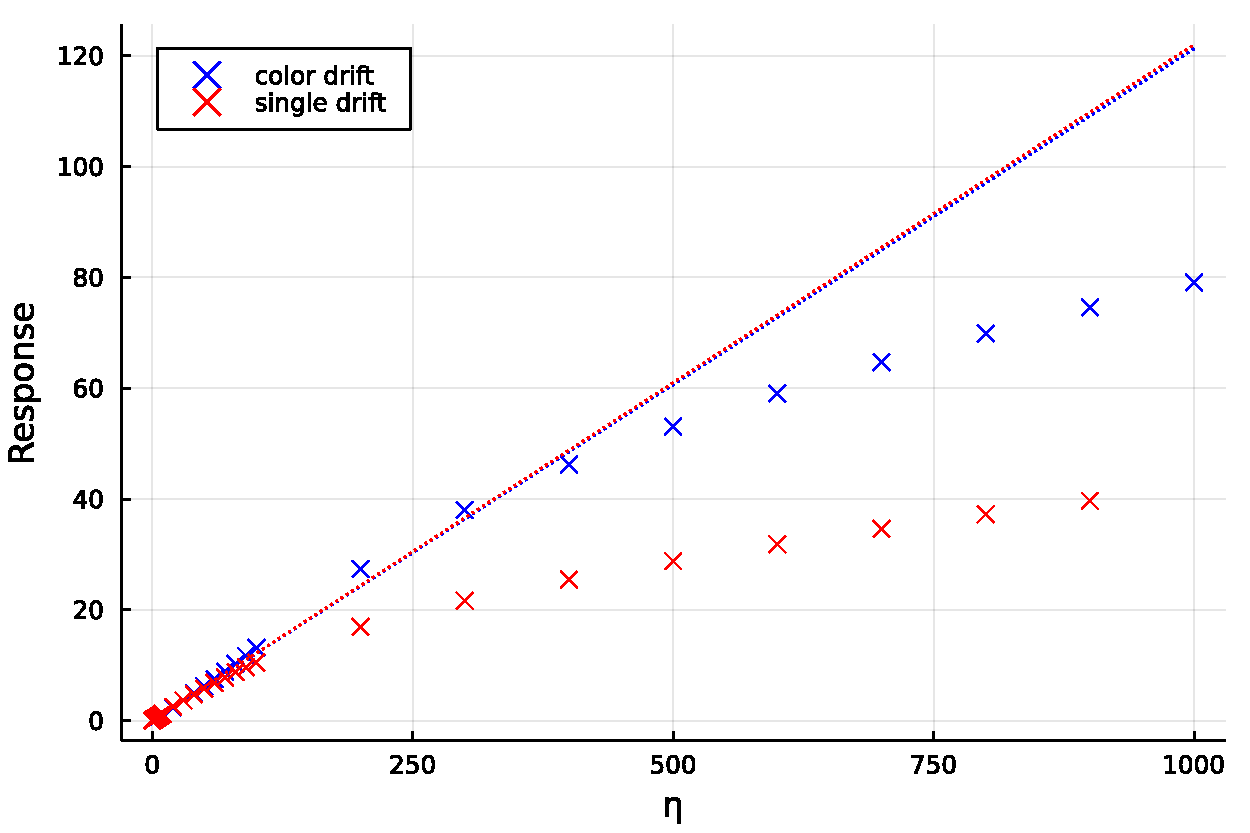
\includegraphics[width=0.7\linewidth]{figures/nemd/nemd_mobility_full.pdf}
      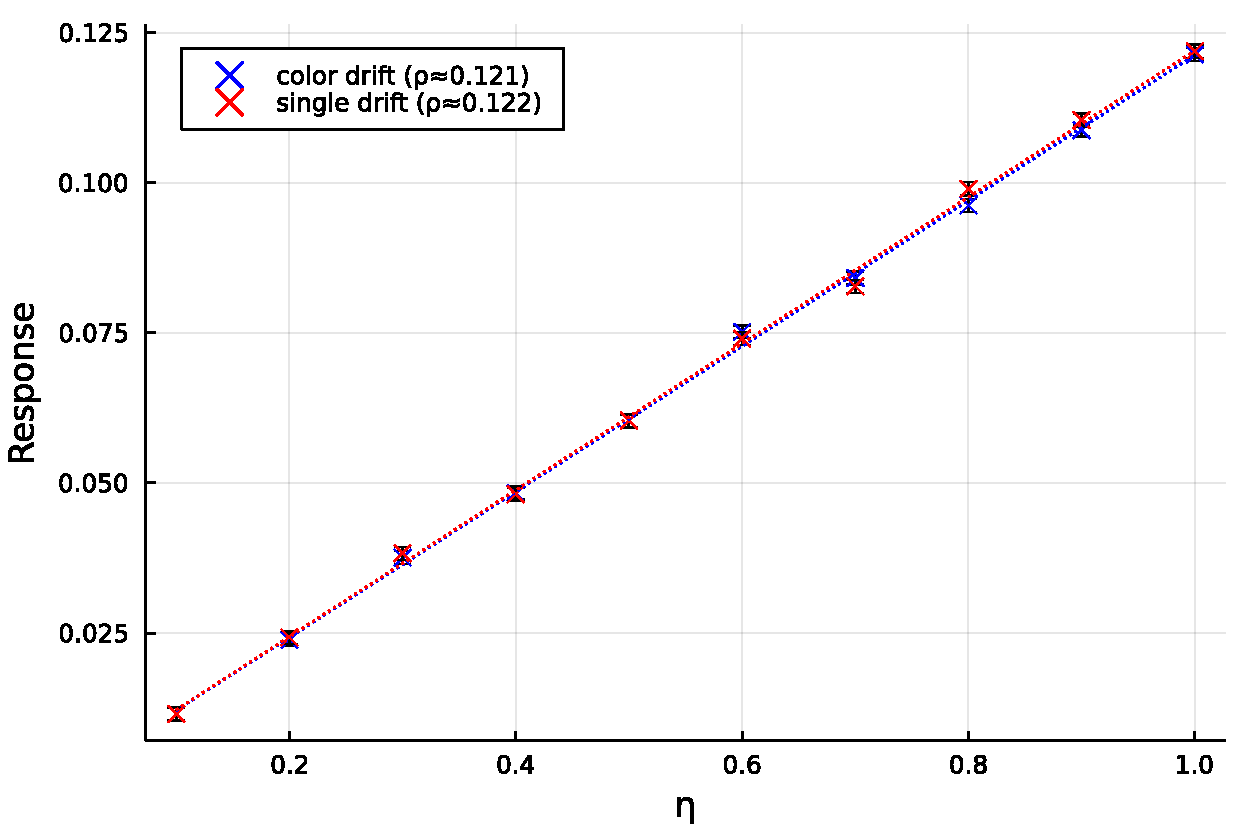
\includegraphics[width=0.7\linewidth]{figures/nemd/nemd_mobility_linear.pdf}
      \caption{ \label{fig:nemd_mobility_full}
        Average mobility response against forcing intensity for the Lennard-Jones system \eqref{eq:reference_thermo_condition}. Extrapolations of the linear response are plotted in dotted lines.
      }
    \end{center}
  \end{figure}
\subsection{Shear viscosity}
As a second example, we discuss the methods of \cite{JS12} for computing shear-viscosity. We refer to this paper for thorough statements and proofs.
Let us assume for notational simplicity that $M=m\Id$.
We consider a case of the dynamics \eqref{eq:general_nemd_dynamics} with a forcing which acts on the longitudinal (x) momenta, and is dependent on the transverse (y) positions.
More precisely, we fix a reference periodic function $F_y:L\mathbb{T}\longrightarrow \R$,
and index the state as \[\left(q_{i\alpha}\right)_{\substack{\leq i\leq N\\1\leq \alpha\leq d}},\qquad \left(p_{i\alpha}\right)_{\substack{\leq i\leq N\\1\leq \alpha\leq d}}.\]
The non-equilibrium dynamics is defined by the following expression for $F$:
\begin{equation}
    \label{eq:shear_viscosity_forcing}
    \forall\, 1\leq i\leq N,\,\forall\, 2\leq \alpha\leq d,\qquad F(q)_{i1}=F_y(q_{i2}),\qquad F(q)_{i\alpha}=0.
\end{equation}
The idea is that by imposing a forcing \textit{profile} in the x-direction, we observe a velocity profile in response, which depends on the $y$-coordinate.
\begin{remark}[Anisotropic friction]
    In fact the precise model considered in \cite{JS12} also imposes a separate friction coefficient $\gamma_x$ for the longitudinal fluctuation-dissipation part of the dynamics.
    This can be interpreted as a simple case of a generalized Langevin dynamics where the friction coefficient $\gamma$ is an anisotropic diagonal matrix, which does not pose any difficulties from the theoretical point of view.
    We therefore restrict our attention to the case where $\gamma$ is scalar.
\end{remark}
More precisely, we define
\begin{equation}
    \label{eq:velocity_profile}
    u_x(Y)\defeq \underset{\epsilon \to 0}{\lim} \, \underset{\eta \to 0}{\lim} \frac{L_y\E_\eta \left[\sum_{i=1}^N p_{i1}\chi_\epsilon(q_{i2}-Y)\right]}{\eta mN}
\end{equation}
to be the linear response profile in the longitudinal velocity, where $(\chi_\epsilon)_{\epsilon>0}$ is an approximation to the identity (that is a sequence of smooth compactly supported test functions which converge to the Dirac delta function in the sense of distributions).
In practice, $u_x$ can be estimated from numerical trajectories by decomposing the domain $\mathcal D$ in a finite number of transverse slices,
 and measuring the average longitudinal velocity in each of these slices.
 The shear viscosity $\sigma$ is then defined by the differential equation
\begin{equation}
    \label{eq:shear_viscosity_relation_diffeq}
    \sigma u_x''(Y)+\gamma \rho u_x(Y)=\rho F_y(Y),
\end{equation}
where $\rho= N/L^3$ is the particle density.
In fact, the solutions to \eqref{eq:shear_viscosity_relation_diffeq} are periodic, thus the magnitude of the linear response can be estimated through Fourier-like coefficients.
This has the advantage of giving an estimation of the linear response in the general framework defined above, and avoiding the discretization error arising from the finite number of transverse slices.
To this effect, we define the response observables as empirical Fourier coefficients (or imaginary parts thereof):
\begin{equation}
    \label{eq:nemd_shear_viscosity_response}
    R_k(q,p)=\frac{1}N\sum_{i=1}^N\frac{p_{i1}}{m}\sin\left(\frac{2k\pi q_{i2}}{L}\right).
\end{equation}
provided $F_y$ is not orthogonal to the family
\[\left\{ y\mapsto \sin\left(\frac{2k\pi y}{L}\right),\,k\geq 1\right\} ,\]
in $L^2([0,L))$, these observables give a meaningful measure of the linear response. In practice, it is sufficient to consider $k=1$ and carefully choose the forcing.
\begin{remark}
    To obtain better statistics, one may for the purpose of numerical simulations want to consider a periodic domain whose unit cell is still a cuboid, but with a side length in the longitudinal direction that is longer than in the transverse direction.
    In this case we simply replace $L$ by $L_y$ in the response observables, where $L_y$ is the length of the unit cell in the transverse direction.
\end{remark}
The shear viscosity can then be computed from equation \eqref{eq:shear_viscosity_relation_diffeq}, given an estimator $\widehat{R}_{k,N_{\mathrm{iter}}}$ of the form \eqref{eq:nemd_response_estimator}, through
\begin{equation}
    \label{eq:shear_viscosity_nemd_estimator}
    \hat{\sigma}_{N_{\mathrm{iter}}}=\rho\left(\frac{F_k}{\widehat{R}_{k,N_{\mathrm{iter}}}}-\gamma\right)\left(\frac{L}{2k\pi}\right)^2,
\end{equation}
again considering $k=1$ in practice.
\section{The Green-Kubo method}
An alternative route to the perturbation method described above leverages a famous expression for the transport coefficient in terms of an integrated correlation function, or, in less prosaic language, in terms of the fluctuations at equilibrium of the response observable.
This is the Green-Kubo method, which we describe in this section. We consider the invariant measure for the non-equilibrium dynamics \eqref{eq:general_nemd_dynamics}. By Theorem \ref{thm:nemd_exst_invariant_measure}, there exists a unique invariant measure with density $\psi_\eta$.
For notational consistency, let us write $\psi_0$ for the density of the equilibrium measure $\mu$. Then the following result holds 
\begin{theorem}[Series expansion for the non-equilibrium steady state]
    \label{thm:nemd_steady_state_series}
    There exists $r>0$ such that for all $0<\eta<r$,
    \begin{equation}
    \label{eq:nemd_steady_state_series}
        \frac{\psi_\eta}{\psi_0}=\left(1+\eta(\widetilde{\cL} \Pi \cL_\gamma^{-1}\Pi)^*\right)^{-1}\1_{\mathcal E}=\left(1+\sum_{k=1}^{\infty}(-\eta)^k\left[(\tilde \cL \Pi\cL_\gamma^{-1}\Pi)^*\right]^k\right)\1_{\mathcal E},
    \end{equation}
    where $\widetilde{\cL}$ is defined by \eqref{eq:nemd_generator}, $\Pi$ is the equilibrium centering projector defined in \eqref{eq:equilibrium_projector}, and the adjoint is taken in $L^2(\mu)$.
\end{theorem}
\begin{proof}[Sketch of proof]
    The second equality identifies the Neumann series on the right as the resolvent of $-(\widetilde{\cL} \Pi \cL_\gamma^{-1}\Pi)^*$, provided $\eta$ is taken small enough.
    In fact, from the spectral theory of bounded operators, $r$ can be determined as the spectral radius of $(\widetilde{\cL} \Pi \cL_\gamma^{-1}\Pi)^*$ in the space of bounded operators $\mathcal{B}(L^2_0(\mu))$.
    The core of the argument lies in making the ansatz
    \begin{equation}
        \label{eq:nemd_measure_ansatz}
        \psi_\eta=\psi_0(1+\eta f_1+\eta^2 f_2+\dotsm).
    \end{equation}
    The stationary Fokker-Planck equation \eqref{eq:nemd_fp_equation} writes
    \[(\cL_\gamma +\eta \widetilde{\cL})^{\dagger}\psi_0(1+\eta f_1+\eta^2 f_2+\dotsm)=(\cL_\gamma +\eta \widetilde{\cL})^{*}(1+\eta f_1+\eta^2 f_2+\dotsm)=0.\]
    By formally separating terms by degree in $\eta$, we obtain
    \begin{align*}
        \cL_\gamma^* \1_\mathcal E&=0,\\
        \widetilde{\cL}^*\1_{\mathcal E}+\cL_\gamma^*f_1&=0,\\
        \widetilde{\cL}^*f_1+\cL_\gamma^*f_2&=0,
    \end{align*}
    and so on. Note that the first equality is the equilibrium Fokker-Planck equation.
    Thus, by induction, again formally, we obtain.
    \begin{align*}
        f_1 &= (-\cL_\gamma^*)^{-1}\widetilde{\cL}^*\1_{\mathcal E},\\
        f_2 &= (-\cL_\gamma^*)^{-1}\widetilde{\cL}^*f_1,\\
        &\dotsm\\
        f_n &= \left[(-\cL_\gamma^*)^{-1}\widetilde{\cL}^*\right]^{n}\1_{\mathcal E},
    \end{align*}
    whence the formal proof follows, by observing that we can write 
    \[(-\cL_\gamma^*)^{-1}\widetilde{\cL}^*=-(\widetilde{\cL} \Pi \cL_\gamma^{-1}\Pi)^*.\]
    For a rigorous proof, several points should be made precise:
    \begin{enumerate}[(i)]
        \item The convergence of the series \eqref{eq:nemd_steady_state_series} for sufficiently small $\eta$, which can be obtained by showing the boundedness of the operator \[(\widetilde{\cL} \Pi \cL_\gamma^{-1}\Pi)^*\] on $L_0(\mu)$.
        \item The fact that \[\psi_0\left(1+\eta(\widetilde{\cL} \Pi \cL_\gamma^{-1}\Pi)^*\right)^{-1}\1_{\mathcal E}\] is indeed a solution to the stationary Fokker-Planck equation.
        \item The fact that it is indeed a probability density. 
    \end{enumerate}
    One can then conclude by unicity of the steady-state measure.
\end{proof}
Strikingly, we can read the linear response directly from the first term of the series expansion.
\begin{corollary}[Green-Kubo formula]
    Let $R$ be any response observable such that $\E_\mu[R]=0$, and $R\in L^{\infty}_{\mathcal{K}_n}$ for some $n$.
    Then we have the following formula for the linear response
    \begin{equation}
        \label{eq:green_kubo}
        \underset{\eta\to 0}{\lim}\,\frac{\E_{\eta}[R]}{\eta}=\int_0^\infty \E_\mu[R(q_t,p_t)S(q_0,p_0)]\dif t,
    \end{equation}
    where the expectation on the right hand side is with respect to all equilibrium dynamics trajectories with canonical initial distribution, and $S$ is defined by
    \begin{equation}
        \label{eq:conjugate_response}
        S=\widetilde{\cL}^*\1_{\mathcal E}=\beta F(q)\cdot M^{-1}p,
    \end{equation}
    and is called the conjugate response function. The latter expression follows from a simple integration by parts.
\end{corollary}
\begin{proof}
    By Theorem \ref{thm:nemd_steady_state_series}, we can write 
    \begin{align*}
        \underset{\eta\to 0}{\lim}\,\frac{\E_{\eta}[R]}{\eta}&=\int_{\mathcal E}R(q,p)(-\cL_\gamma^*)^{-1}\widetilde{\cL}^*\1_{\mathcal E}\psi_0(q,p)\,\dif q\, \dif p\\
        &=\int_{\mathcal E}(-\cL_\gamma)^{-1}R(q,p)S(q,p)\psi_0(q,p)\,\dif q\, \dif p\\
        &=\int_{\mathcal E}\int_0^\infty\E^{(q,p)}[R(q_t,p_t)S(q_0,p_0)]\psi_0(q,p)\,\dif t\,\dif q\,\dif p\\
        &=\int_0^\infty \E_\mu[R(q_t,p_t)S(q_0,p_0)]\,\dif t,
    \end{align*}
    where we rely on an expression like \eqref{eq:resolvent_langevin} for $(-\cL_\gamma)^{-1}.$
\end{proof}
The Green-Kubo formula has a great advantage, in that it allows us to estimate the transport coefficients for as many different perturbations and response observables as we want \textbf{from a single equilibrium trajectory}.
Indeed, one only needs to compute the corresponding integrated correlation functions \eqref{eq:green_kubo}.
\subsection{Numerical implementation}
We now describe a method to compute correlation functions necessary to the Green-Kubo method from a single long numerical trajectory.
This method is described by Tuckerman in \cite{T10}, section 13.4.2 for Hamiltonian trajectories.
In fact we consider a slight extension in which we let $R$ and $S$ to be vector-valued observables.
For notational simplicity, we assume that $R$ and $S$ are component-wise centered. The quantities we want to estimate are 
\begin{equation}
    \label{eq:time_correlation}
    C(t)=\E_\mu[R(q_t,p_t)^\intercal S(q_0,p_0)]
\end{equation}
we let $(q^n,p^n)_{n\geq 0}$ be a numerical trajectory, which we see as the random iterates of the Markov chain associated with a numerical scheme, with a regular timestep $\Dt>0$.
We further assume that the trajectory is stationary for this Markov chain, which is a realistic assumption if we take care of equilibriating the system using our numerical scheme before recording states.
By stationarity, the equality in law
\[(q^n,p^n,q^0,p^0) \overset{\mathrm{law}}{=}(q^{n+k},p^{n+k}q^k,p^k)\]
for all $k$. Hence we define the following estimator for $C(n\Dt)$, for $0\leq n\leq N_{\mathrm{iter}}:$
\begin{equation}
    \label{eq:ac_estimator}
    \widehat{C}_{N_{\mathrm{iter}}}(n\Dt) = \frac{1}{N_{\mathrm{iter}}-n+1}\sum_{k=0}^{N_{\mathrm{iter}}-n}R(q^{n+k},p^{n+k})^\intercal S(q^k,p^k).
\end{equation}
Note the quality of these estimators degrades with $n$. Thus in practice, we fix $N_{\mathrm{corr}}\ll N_{\mathrm{iter}}$, and compute these estimators for $0\leq n \leq N_{\mathrm{corr}}$.
For implementation details, we refer to the Appendix and links therein to relevant Julia code.

Using these estimators, we can estimate the transport coefficient through the Green-Kubo formula \eqref{eq:green_kubo}. The simplest way is to use a naive Riemann sum, or rectangle rule:
\[\rho_F \approx \Dt\sum_{k=0}^{N_{\mathrm{corr}}} \widehat{C}_{N_{\mathrm{iter}}}(k\Dt).\]
In fact, analysis shows that using a trapezoidal rule reduces the error.
However, these procedures introduce a truncation in time of the integral in \eqref{eq:green_kubo}.
Another approach consists of extrapolating the behavior of $\widehat{C}_{N_{\mathrm{iter}}}$ by fitting a parametric model 
\begin{equation}
    \label{eq:time_correlation_parametric_model}
    C_{\theta}(t)=\e^{-\lambda t}\left(\sum_{k=1}^{m}a_k\sin(f_k t+\omega_k)\right),
\end{equation}
where \[\theta=(\lambda,a_1,f_1,\omega_1,\dots,a_m,f_m,\omega_m)\in \R_{>0}\times\R^{3m}\]
is the parameter. The form of this model is justified empirically, although a formal argument based on a diagonalisation of the evolution semi-group can be made. 
Rigorously justifying and quantifying the accuracy of this model requires fine knowledge of the spectrum of $\cL_\gamma$.
At any rate, we can then fit the model in a least-squares sense,
\begin{equation}
    \theta^*=\underset{\theta\in \R_{>0}\times\R^{3m}}{\mathrm{argmin}}\sum_{n=0}^{N_{\mathrm{corr}}}\left| C_{\theta}(n\Dt)-\widehat{C}_{N_{\mathrm{iter}}}(n\Dt) \right|^2,
\end{equation}
for instance using gradient descent, and deduce the estimator for the transport coefficient,
\begin{equation}
    \label{eq:rho_F_estimator_GK_fit}
    \widehat{\rho}^{\mathrm{GK}}_{F,N_{\mathrm{iter}}}=\int_0^\infty C_{\theta^*}(t)\,\dif t,
\end{equation}
leveraging the elementary identity
\begin{equation}
    \label{eq:int_analytic_form}
    \int_0^{\infty}\e^{-\lambda t}a\sin(ft+\omega)\,\dif t=a\frac{\lambda\cos\omega-f\sin\omega}{f^2+\lambda^2}.
\end{equation}
\subsection{Mobility}
\subsection{Shear viscosity}
\chapter{Norton methods}
\section{Introduction}
So far, the non-equilibrium setting we considered was one in which we perturbed the dynamics by a constant forcing,
 and measured the linear relationship between the magnitude of the forcing and the induced response.
An alternative idea would be to consider fixing the response, and measuring the magnitude of the forcing needed to induce it. This is the core of the Norton method.


\section{Norton dynamics for the mobility observable}
Let us fix a direction defined by a vector $F\in \R^{dN}$. The response we consider is the velocity in the direction $F$, which is the observable \[F\cdot \left(M^{-1} p\right).\]
Again, we consider perturbed Langevin dynamics, but this time the magnitude of the non-gradient force $\eta$ is replaced by a fluctuating magnitude $\Lambda_t$, which is determined in order to ensure that the response
\[v=F\cdot\left(M^{-1}p\right)=p\cdot\left(M^{-1}F\right)\]
is a constant.

\subsection{The dynamics}
Thus, we consider the dynamics
\begin{equation}
    \label{eq:norton_method}
    \left\{\begin{aligned}
        \dif q_t&=\left(M^{-1}p_t\right)\dif t\\
        \dif p_t&=-\nabla V(q_t)\dif t -\gamma\left(M^{-1}p_t\right)\dif t+\sqrt{\frac{2\gamma}\beta}\dif W_t+F\dif \Lambda_t,
    \end{aligned}\right.
\end{equation}
where $\Lambda_t$ is a real-valued stochastic process. We make the tacit assumption that for fixed $v$, the process $\Lambda_t$ is well-defined and that ergodic averages
\[\frac1 T\int_0^T \dif\Lambda_t=\frac{\Lambda_T-\Lambda_0}T\]
converge almost surely to some average value $R_v$ under an invariant measure for the dynamics. We can easily write an equation for $\Lambda_t$, as follows.
Our aim is to determine
\[\underset{v\to 0}\lim \frac{v}{R_v}\]
Using Itô's formula on the response, we get
\begin{equation}
    \label{eq:formula_response}
\dif \left(\left(M^{-1}F\right)\cdot p\right)_t=\left(M^{-1}F\right)\cdot\left(-\nabla V(q_t)\dif t -\gamma M^{-1}p_t\dif t+\sqrt{\frac{2\gamma}\beta}\dif W_t\right)+\left( \left(M^{-1}F\right)\cdot F\right)\dif\Lambda_t=0,
\end{equation}
which gives $\Lambda_t$ as an Itô process,
\begin{equation}
    \label{eq:norton_multiplier_ito_decomposition}
    \dif \Lambda_t=\left( \left(M^{-1}F\right)\cdot F\right)^{-1}\left(M^{-1}F\right)\cdot\left(\nabla V(q_t)\dif t +\gamma M^{-1}p_t\dif t-\sqrt{\frac{2\gamma}\beta}\dif W_t\right).
\end{equation}
At this point, let us introduce the linear maps
\begin{equation}
    \label{eq:norton_projector}
    \begin{aligned}
        &P_{M,F}\,u=\frac{\left(M^{-1}F\right)\cdot u}{\left(M^{-1}F\right)\cdot F}F\qquad\forall\,u\in\R^{dN}\\
        &P_{M,F}^\perp=\Id-P_{M,F}
    \end{aligned}
\end{equation}
which are simply the orthogonal projectors onto the subspace spanned by $F$ and its orthogonal complement, with respect to the weighted scalar product
\begin{equation}
    \label{eq:norton_weighted_scalar_product}
    \left\langle x,y\right\rangle_{M}=\left\langle M^{-1}x,y\right\rangle.
\end{equation}
Using this projector and substituting $\dif \Lambda_t$ for its value, we get the equation for the augmented dynamics $(q_t,p_t,\Lambda_t)\in \mathcal E\times \R$.
\begin{equation}
    \label{eq:norton_final_sde}
    \left\{\begin{aligned}
        \dif q_t &= M^{-1}p_t\dif t\\
        \dif p_t &= P_{M,F}^\perp\left(-\nabla V(q_t)\dif t -\gamma M^{-1}p_t\dif t +\sqrt{\frac{2\gamma}\beta}\dif W_t\right)\\
        \dif \Lambda_t &=\frac{M^{-1}F}{\left(M^{-1}F\right)\cdot F}\cdot\left(\nabla V(q_t)\dif t +\gamma M^{-1}p_t\dif t-\sqrt{\frac{2\gamma}\beta}\dif W_t\right)
    \end{aligned}\right.
\end{equation}
Notice this equation is almost the same as for the Langevin dynamics.
The kinetic part is projected onto the $F$-subspace with respect to $\langle \cdot,\cdot\rangle_M$, and $\dif\Lambda_t$ is minus the coordinate in the $F$ direction of the standard Langevin equation for $\dif p_t$, again with respect to $\langle \cdot ,\cdot \rangle_M$.
The Brownian motions $W_t$ are the same in the last two equations, hence $p_t$ and $\Lambda_t$ are coupled processes.[GENERATOR FOR THE FULL DYNAMICS?]

\begin{equation}
    \label{eq:norton_generator}
---
\end{equation}

\subsection{Analytic calculations for the kinetic dynamics}

The kinetic part of the dynamics writes as the combination of a ballistic Hamiltonian evolution
\begin{equation}
    \label{eq:elem_hamiltonian_equation}
    \left\{\begin{aligned}
        \dif q_t&=0\\
        \dif p_t&=-P_{M,F}^\perp\nabla V(q_t)
    \end{aligned}\right.\implies\left\{\begin{aligned}
        q_t&=q_0\\
        p_t&=p_0-tP_{M,F}^\perp\nabla V(q_0)
    \end{aligned}\right.
\end{equation}
and a fluctuation-dissipation part,
\begin{equation}
    \label{eq:projected_OU}
    \dif p_t=-\gamma P_{M,F}^\perp M^{-1}p_t\dif t-\sqrt{\frac{2\gamma}{\beta}}P_{M,F}^\perp\dif W_t,
\end{equation}
which can also be analytically solved.
Indeed, applying Itô's formula to the rescaled process $\e^{\gamma P_{M,F}^\perp M^{-1}t}p_t$ yields
\[\mathrm{e}^{\gamma P_{M,F}^\perp M^{-1}t}\left(\gamma P_{M,F}^\perp M^{-1}p_t\dif t - \gamma P_{M,F}^\perp M^{-1}p_t\dif t-\sqrt{\frac{2\gamma}{\beta}} P_{M,F}^\perp\dif W_t\right),\]
hence we get 
\begin{equation}
    \label{eq:projected_ou_analytical_form}
    \begin{aligned}
    p_t&=\mathrm{e}^{-\gamma P_{M,F}^\perp M^{-1}t}p_0-\sqrt{\frac{2\gamma}{\beta}}\int_0^t\mathrm{e}^{\gamma P_{M,F}^\perp M^{-1}(s-t)} P_{M,F}^\perp\dif W_s\\
    &=\mathrm{e}^{-\gamma P_{M,F}^\perp M^{-1}t}p_0-\sqrt{\frac{2\gamma}{\beta}}\left(\int_0^t\e^{-\gamma P_{M,F}^\perp M^{-1}s}P_{M,F}^\perp\e^{-\gamma P_{M,F}^\perp M^{-1}s} \dif s\right)^{\frac12}G,
    \end{aligned}
\end{equation}
where the last equality holds in law if $G$ is a standard $dN$-dimensional Gaussian, using Itô's isometry and the symmetry of $\e^{\gamma P_{M,F}^\perp M^{-1}t}$ for all $t$.
The matrix exponentials and integrals can be computed, however there is no concise expression like \eqref{eq:propagators} because $P_{M,F}^\perp M^{-1}$ is not invertible.

In the case of a homogeneous system with $M=\alpha\Id$ (in which case we can assume by a judicious choice of mass unit that $M=\Id$), a more concise expression can be found, using the identity
\[\e^{r\Pi}=\sum_{k=0}^\infty \frac{r^k}{k!}\Pi^k=\Id+\left(\sum_{k=1}^\infty\frac{r^k}{k!}\right)\Pi=\Id+\left(\e^r-1\right)\Pi.\]
This identity follows, for $\Pi$ a linear projector, from applying the projector identity \[\Pi=\Pi^2=\Pi^3=\dotsm.\]
We write the following derivation in the case of a general projector $\Pi$, and conclude by taking the case $\Pi=P_{M,F}^\perp$. We also note $\Pi^\perp=\Id-\Pi$.

\begin{equation}
    \begin{aligned}
        \mathrm{e}^{-\gamma \Pi t}p_0-\sqrt{\frac{2\gamma}{\beta}} \Pi\left(\int_0^t\e^{2\gamma s \Pi }\dif s\right)^{\frac12}G&=\left(\Id+\left(\e^{-\gamma t}-1\right)\Pi\right)p_0-\sqrt{\frac{2\gamma}{\beta}}\Pi\left(\int_0^t\left(\Id+\left(\e^{-2\gamma s}-1\right)\Pi\right)\dif s\right)^\frac{1}{2}G\\
        &=\left(\Pi^\perp +\e^{-\gamma t}\Pi\right)p_0-\sqrt{\frac{2\gamma}{\beta}}\Pi\left(t\Pi^\perp+\frac{1-\e^{-2\gamma t}}{2\gamma}\Pi\right)^{\frac 12}G.
    \end{aligned}
\end{equation}
Now, observe that $\R^{dN}$ writes as the sum of two orthogonal spaces, each of which is an eigenspace for both $\Pi$ and $\Pi^\perp$, and correspond respectively to the eigenvalues $0$ and $1$ (this correspondence being flipped upon passing from $\Pi$ to $\Pi^\perp$). By an easy spectral calculation, we also have $\Pi^\alpha=\Pi$ for any $\alpha>0$,
which allows to conclude that 
\[(a\Pi^\perp+b\Pi)^\alpha=a^\alpha\Pi^\perp+b^\alpha\Pi\qquad \forall\,a,b,\alpha>0,\]
and finally
\begin{equation}
    \label{eq:norton_ou_solved_no_mass}
    \begin{aligned}
    \mathrm{e}^{-\gamma \Pi t}p_0-\sqrt{\frac{2\gamma}{\beta}} \Pi\left(\int_0^t\e^{2\gamma s \Pi }\dif s\right)^{\frac12}G&=\Pi^\perp p_0+\e^{-\gamma t}\Pi p_0-\sqrt{\frac{2\gamma t}{\beta}}\Pi\Pi^\perp G-\sqrt{\frac{1-\e^{-2\gamma t}}{\beta}}\Pi G\\
    &=\Pi^\perp p_0+\e^{-\gamma t}\Pi p_0-\sqrt{\frac{1-\e^{-2\gamma t}}{\beta}}\Pi G,
    \end{aligned}
\end{equation}
where we use $\Pi\Pi^\perp=0$ for the last equality.
Comparing equation \eqref{eq:norton_ou_solved_no_mass} and equation \eqref{eq:propagators} yields a clear interpretation of the action of the fluctuation-dissipation term on the dynamics: there is no effect in the direction tangent to $F$, and a standard Ornstein-Uhlenbeck process applies to the dynamics projected onto the subspace orthogonal to $F$ (note $\Pi G$ can then be viewed as a $(dN-1)$-dimensional standard Gaussian by isotropy).
We also note that a similar computation may be performed in the case where both $M$ and $P_{M,F}$ are simultaneously diagonalizable, for instance if $M$ is a diagonal matrix and $F$ has a single non-zero component.

\section{Splitting schemes}
Consider the Norton dynamics on the state variable $(q_t,p_t)$. Its generator is given by the operator

\begin{equation}
    \label{eq:norton_generator}
    \cL_F\varphi(q,p)=(M^{-1}p)\cdot \nabla_q\varphi(q,p)-(P_{M,F}^\perp\nabla V(q)-\gamma P_{M,F}^\perp M^{-1}p)\cdot\nabla_p\varphi(q,p)-\frac{\gamma}\beta\mathrm{Tr}\left(P_{M,F}^\perp\nabla_p^2\varphi(q,p)\right),
\end{equation}
which we rewrite as 
\begin{equation}
    \label{eq:norton_generator_splitting}
    \cL_F=A+B_F+\gamma C_F,\qquad \text{with} \qquad
    \left\{\begin{aligned}
        B_F\varphi(q,p)&=\left(P_{M,F}^\perp\nabla V(q)\right)\cdot \nabla_p\varphi(q,p)\\
        C_F\varphi(q,p)&=-\left(P_{M,F}^\perp M^{-1}p\right)\cdot\nabla_p\varphi(q,p)+\frac1\beta\mathrm{Tr}\left(P_{M,F}^\perp\nabla_p^2\varphi(q,p)\right).
    \end{aligned}\right.
\end{equation}
The $A$ and $B_F$ operators are the generators of exactly integrable dynamics (namely ballistic Hamiltonian dynamics), and $C_F$ generates an analytically solvable diffusion process given in \eqref{eq:projected_ou_analytical_form}. Hence we can use a splitting scheme exactly as we did in the case of the Langevin dynamics, as discussed in section \ref{section:splitting_schemes_langevin}. 
We will use the exact same terminology in this context, referring to a scheme by the order in which the elementary dynamics are integrated.
For instance, the BAO scheme associated with the Norton dynamics for $F$ is the following. We fix a timestep $\Dt>0$.

\begin{example}[Norton BAO scheme]
    \begin{equation}
        \left\{
            \begin{aligned}
                p^{n+\frac12}&=p^n-\Dt P_{M,F}^\perp \nabla V(q^n)\\
                q^{n+1}&=q^n+\Dt M^{-1}p^{n+\frac12}\\
                p^{n+1}&=\mathrm{e}^{-\gamma P_{M,F}^\perp M^{-1}\Dt}p^{n+\frac12}-\sqrt{\frac{2\gamma}{\beta}}\left(\int_0^\Dt\e^{-\gamma P_{M,F}^\perp M^{-1}s}P_{M,F}^\perp\e^{-\gamma P_{M,F}^\perp M^{-1}s} \dif s\right)^{\frac12}G^n
            \end{aligned}\right.
    \end{equation}
\end{example}
The $\gamma C_F$-step is cumbersome to write in full, but it is always of the form 
\[p^{n+1}=R_\Dt p^n + S_\Dt G^n\]
for fixed matrices $R_\Dt$ and $S_\Dt$ which only have to be computed once.

\section{Estimating transport coefficients}
To estimate the transport coefficient $\rho_F$ using this method, we need to estimate the average forcing. Recalling the SDE \eqref{eq:norton_final_sde} for $\dif \Lambda$, the martingale term involving the Brownian motion cancels out under steady-state averaging.
Hence we can estimate the average forcing using the following ergodic average:
\begin{equation}
    \label{eq:norton_ergodic_forcing}
    \frac{1}T\int_0^T\frac{M^{-1}F}{\left(M^{-1}F\right)\cdot F}\cdot\left(\nabla V(q_t)+\gamma M^{-1}p_t\right)\dif t.
\end{equation}
In the case of a mass matrix $M=m\Id$ and $|F|=1$, which we now assume on to lighten notation, this becomes
\begin{equation}
    \label{eq:norton_ergodic_forcing_homogeneous}
    \frac{1}{T}\int_0^T F\cdot\left(\nabla V(q_t)\right)\dif t + \gamma v,
\end{equation}
using the expression for the response, so that the finite difference estimator of $\rho_F$ is given by
\begin{equation}
    \label{eq:norton_transport estimator}
    \widehat{\rho}_{F,T}=\frac{v}{\gamma v+\frac{1}{T}\int_0^T F\cdot\left(\nabla V(q_t)\right)\dif t}.
\end{equation}
In practice, we approximate the continuous ergodic average in the denominator by discrete averages.
\chapter*{Performance analysis}

\end{document}